\documentclass[
]{jss}

\usepackage[utf8]{inputenc}

\providecommand{\tightlist}{%
  \setlength{\itemsep}{0pt}\setlength{\parskip}{0pt}}

\author{
Rebecca Fisher\\Australian Institute of Marine Science, Crawley, WA,
Australia \And Diego Barneche\\Australian Institute of Marine Science,
Crawley, WA, Australia \And Gerard Ricardo\\Australian Institute of
Marine Science, Townsville, Qld, Australia \And David
Fox\\Environmetrics Australia, Beaumaris, Victoria, Australia
}
\title{\pkg{bayesnec}: An R Package for C-R Modelling and Estimation of
No-Effect-Concentrations}

\Plainauthor{Rebecca Fisher, Diego Barneche, Gerard Ricardo, David Fox}
\Plaintitle{bayesnec: An R Package for C-R Modelling and Estimation of
No-Effect-Concentrations}
\Shorttitle{C-R Modelling With \pkg{bayesnec}}

\Abstract{
The pkg\{bayesnec\} package in R has been developed to fit
concentration(dose) - response curves (C-R) to toxicity data for the
purpose of deriving no-effect-concentration (\emph{NEC}),
no-significant-effect-concentration (\emph{NSEC}), and
effect-concentration (of specified percentage `x', \emph{ECx})
thresholds from non-linear models fitted using Bayesian MCMC fitting
methods via pkg\{brms\} \citep{Burkner2017, Burkner2018} and
pkg\{rstan\} \citep{rstan2020}. In pkg\{bayesnec\} it is possible to fit
a single model, custom model-set, specific model-set or all of the
available models. When multiple models are specified the \texttt{bnec}
function returns a model weighted average estimate of predicted
posterior values. A range of support functions and methods are also
included to work with the returned single, or multi- model objects that
allow extraction of raw, or model averaged predicted, \emph{ECx},
\emph{NEC} and \emph{NSEC} values and to interrogate the fitted model or
model-set. The statistical methods used mean that the uncertainty in
derived threshold values can be robustly quantified, including
uncertainty in individual model fits to the underlying observed data, as
well as uncertainty in the model functional form.
}

\Keywords{ecotoxicology, effect concentration, threshold
derivation, nec, \proglang{brms}}
\Plainkeywords{ecotoxicology, effect concentration, threshold
derivation, nec, brms}

%% publication information
%% \Volume{50}
%% \Issue{9}
%% \Month{June}
%% \Year{2012}
%% \Submitdate{}
%% \Acceptdate{2012-06-04}

\Address{
        }

% Pandoc citation processing

% Pandoc header

\usepackage{amsmath}

\begin{document}

\hypertarget{introduction}{%
\section{Introduction}\label{introduction}}

Concentration-response (C-R) modelling is fundamental to assessing
toxicity and deriving toxicity thresholds used in the risk assessments
that underpin protection of human health and the environment. It is
widely used in the disciplines of pharmacology, toxicology and
ecotoxicology. Typically C-R curves are non-linear, which increases the
complexity of model fitting. Estimates of uncertainty in parameters and
derived thresholds are critical to effective integration in risk
assessment and formal decision frameworks. Bayesian methods that allow
robust quantification of uncertainty with intuitive and direct
probabilistic meaning \citep{Ellison1996} and are therefore an ideal
platform for C-R modelling in most settings.

Bayesian model fitting can be difficult to automate across a broad range
of usage cases, particularly with respect to specifying valid initial
parameter values and appropriate priors. This is one reason the use of
Bayesian statistics for \emph{NEC} estimation (or even \emph{ECx}
estimation) is not currently widely adopted across the broader
ecotoxicology and toxicology communities, who may not have access to
specialist statistical expertise. The pkg\{bayesnec\} package provides
an accessible interface specifically for fitting \emph{NEC} and other
C-R models using Bayesian methods. A range of models can be specified
based on the known distribution of the ``concentration'' or ``dose''
variable (the predictor, x) as well as the ``response'' (y) variable.
The model formula, including priors and initial values required to call
pkg\{brms\} are automatically generated based on information contained
in the supplied data.

\hypertarget{technical-details-and-usage}{%
\section{Technical details and
Usage}\label{technical-details-and-usage}}

This project started with an implementation of the \emph{NEC} model
based on that described in \citep{Fox2010, Pires2002} using R2jags
\citep{Su2015}. Code for fitting this initial model was developed into
the R package pkg\{jagsNEC\} and expanded to include several C-R models
and further generalised to allow a large range of response variables to
be modelled using their appropriate statistical distribution. While the
original pkg\{jagsNEC\} implementation supported Gaussian, Poisson,
Binomial, Gamma, Negative-binomial and Beta response data,
pkg\{bayesnec\} supports all of these in addition to the Beta-binomial
family. Furthermore, the new structure implemented using pkg\{brms\}
means pkg\{bayesnec\} can be readily extended to include any of the
pkg\{brms\} families. In addition to greater flexibility in the
available response families, pkg\{bayesnec\} includes a larger range of
alternative \emph{NEC} model types, as well as most typically used
smooth C-R models (such as 4-parameter logistic and Weibull models) that
have no \emph{NEC} `step' function but simply model the response as a
smooth function of concentration. We have now incorporated most of the
commonly used models in frequentist packages such as pkg\{drc\}
\citep{Ritz2016} (please see the
\href{https://open-aims.github.io/bayesnec/articles/example2b.html}{Model
details} vignette for more information on the full list of models
currently available in pkg\{bayesnec\}).

\hypertarget{model-specification}{%
\subsection{Model specification}\label{model-specification}}

The main working function in pkg\{bayesnec\} is \texttt{bnec}. We have
attempted to make the \texttt{bnec} function as easy to use as possible,
targeting the novice R user. A pkg\{bayesnec\} model can be fit as
simply as:

\begin{CodeChunk}
\begin{CodeInput}
R> library(bayesnec)
R> data(nec_data)
R> exmp_fit <- bnec(data = nec_data, x_var = "x", y_var = "y", model = "all")
\end{CodeInput}
\begin{CodeOutput}

SAMPLING FOR MODEL '2efdac7dae678c639f889f765ec41be7' NOW (CHAIN 1).
Chain 1: 
Chain 1: Gradient evaluation took 0 seconds
Chain 1: 1000 transitions using 10 leapfrog steps per transition would take 0 seconds.
Chain 1: Adjust your expectations accordingly!
Chain 1: 
Chain 1: 
Chain 1: Iteration:    1 / 10000 [  0%]  (Warmup)
Chain 1: Iteration: 1000 / 10000 [ 10%]  (Warmup)
Chain 1: Iteration: 2000 / 10000 [ 20%]  (Warmup)
Chain 1: Iteration: 3000 / 10000 [ 30%]  (Warmup)
Chain 1: Iteration: 4000 / 10000 [ 40%]  (Warmup)
Chain 1: Iteration: 5000 / 10000 [ 50%]  (Warmup)
Chain 1: Iteration: 6000 / 10000 [ 60%]  (Warmup)
Chain 1: Iteration: 7000 / 10000 [ 70%]  (Warmup)
Chain 1: Iteration: 8000 / 10000 [ 80%]  (Warmup)
Chain 1: Iteration: 9000 / 10000 [ 90%]  (Warmup)
Chain 1: Iteration: 9001 / 10000 [ 90%]  (Sampling)
Chain 1: Iteration: 10000 / 10000 [100%]  (Sampling)
Chain 1: 
Chain 1:  Elapsed Time: 42.987 seconds (Warm-up)
Chain 1:                6.822 seconds (Sampling)
Chain 1:                49.809 seconds (Total)
Chain 1: 

SAMPLING FOR MODEL '2efdac7dae678c639f889f765ec41be7' NOW (CHAIN 2).
Chain 2: 
Chain 2: Gradient evaluation took 0 seconds
Chain 2: 1000 transitions using 10 leapfrog steps per transition would take 0 seconds.
Chain 2: Adjust your expectations accordingly!
Chain 2: 
Chain 2: 
Chain 2: Iteration:    1 / 10000 [  0%]  (Warmup)
Chain 2: Iteration: 1000 / 10000 [ 10%]  (Warmup)
Chain 2: Iteration: 2000 / 10000 [ 20%]  (Warmup)
Chain 2: Iteration: 3000 / 10000 [ 30%]  (Warmup)
Chain 2: Iteration: 4000 / 10000 [ 40%]  (Warmup)
Chain 2: Iteration: 5000 / 10000 [ 50%]  (Warmup)
Chain 2: Iteration: 6000 / 10000 [ 60%]  (Warmup)
Chain 2: Iteration: 7000 / 10000 [ 70%]  (Warmup)
Chain 2: Iteration: 8000 / 10000 [ 80%]  (Warmup)
Chain 2: Iteration: 9000 / 10000 [ 90%]  (Warmup)
Chain 2: Iteration: 9001 / 10000 [ 90%]  (Sampling)
Chain 2: Iteration: 10000 / 10000 [100%]  (Sampling)
Chain 2: 
Chain 2:  Elapsed Time: 43.618 seconds (Warm-up)
Chain 2:                8.325 seconds (Sampling)
Chain 2:                51.943 seconds (Total)
Chain 2: 

SAMPLING FOR MODEL '2efdac7dae678c639f889f765ec41be7' NOW (CHAIN 3).
Chain 3: 
Chain 3: Gradient evaluation took 0 seconds
Chain 3: 1000 transitions using 10 leapfrog steps per transition would take 0 seconds.
Chain 3: Adjust your expectations accordingly!
Chain 3: 
Chain 3: 
Chain 3: Iteration:    1 / 10000 [  0%]  (Warmup)
Chain 3: Iteration: 1000 / 10000 [ 10%]  (Warmup)
Chain 3: Iteration: 2000 / 10000 [ 20%]  (Warmup)
Chain 3: Iteration: 3000 / 10000 [ 30%]  (Warmup)
Chain 3: Iteration: 4000 / 10000 [ 40%]  (Warmup)
Chain 3: Iteration: 5000 / 10000 [ 50%]  (Warmup)
Chain 3: Iteration: 6000 / 10000 [ 60%]  (Warmup)
Chain 3: Iteration: 7000 / 10000 [ 70%]  (Warmup)
Chain 3: Iteration: 8000 / 10000 [ 80%]  (Warmup)
Chain 3: Iteration: 9000 / 10000 [ 90%]  (Warmup)
Chain 3: Iteration: 9001 / 10000 [ 90%]  (Sampling)
Chain 3: Iteration: 10000 / 10000 [100%]  (Sampling)
Chain 3: 
Chain 3:  Elapsed Time: 43.884 seconds (Warm-up)
Chain 3:                5.725 seconds (Sampling)
Chain 3:                49.609 seconds (Total)
Chain 3: 

SAMPLING FOR MODEL '2efdac7dae678c639f889f765ec41be7' NOW (CHAIN 4).
Chain 4: 
Chain 4: Gradient evaluation took 0 seconds
Chain 4: 1000 transitions using 10 leapfrog steps per transition would take 0 seconds.
Chain 4: Adjust your expectations accordingly!
Chain 4: 
Chain 4: 
Chain 4: Iteration:    1 / 10000 [  0%]  (Warmup)
Chain 4: Iteration: 1000 / 10000 [ 10%]  (Warmup)
Chain 4: Iteration: 2000 / 10000 [ 20%]  (Warmup)
Chain 4: Iteration: 3000 / 10000 [ 30%]  (Warmup)
Chain 4: Iteration: 4000 / 10000 [ 40%]  (Warmup)
Chain 4: Iteration: 5000 / 10000 [ 50%]  (Warmup)
Chain 4: Iteration: 6000 / 10000 [ 60%]  (Warmup)
Chain 4: Iteration: 7000 / 10000 [ 70%]  (Warmup)
Chain 4: Iteration: 8000 / 10000 [ 80%]  (Warmup)
Chain 4: Iteration: 9000 / 10000 [ 90%]  (Warmup)
Chain 4: Iteration: 9001 / 10000 [ 90%]  (Sampling)
Chain 4: Iteration: 10000 / 10000 [100%]  (Sampling)
Chain 4: 
Chain 4:  Elapsed Time: 42.038 seconds (Warm-up)
Chain 4:                6.791 seconds (Sampling)
Chain 4:                48.829 seconds (Total)
Chain 4: 

SAMPLING FOR MODEL 'b0b27cbb9362e51885d46d6ec97b2d76' NOW (CHAIN 1).
Chain 1: 
Chain 1: Gradient evaluation took 0.001 seconds
Chain 1: 1000 transitions using 10 leapfrog steps per transition would take 10 seconds.
Chain 1: Adjust your expectations accordingly!
Chain 1: 
Chain 1: 
Chain 1: Iteration:    1 / 10000 [  0%]  (Warmup)
Chain 1: Iteration: 1000 / 10000 [ 10%]  (Warmup)
Chain 1: Iteration: 2000 / 10000 [ 20%]  (Warmup)
Chain 1: Iteration: 3000 / 10000 [ 30%]  (Warmup)
Chain 1: Iteration: 4000 / 10000 [ 40%]  (Warmup)
Chain 1: Iteration: 5000 / 10000 [ 50%]  (Warmup)
Chain 1: Iteration: 6000 / 10000 [ 60%]  (Warmup)
Chain 1: Iteration: 7000 / 10000 [ 70%]  (Warmup)
Chain 1: Iteration: 8000 / 10000 [ 80%]  (Warmup)
Chain 1: Iteration: 9000 / 10000 [ 90%]  (Warmup)
Chain 1: Iteration: 9001 / 10000 [ 90%]  (Sampling)
Chain 1: Iteration: 10000 / 10000 [100%]  (Sampling)
Chain 1: 
Chain 1:  Elapsed Time: 57.153 seconds (Warm-up)
Chain 1:                8.157 seconds (Sampling)
Chain 1:                65.31 seconds (Total)
Chain 1: 

SAMPLING FOR MODEL 'b0b27cbb9362e51885d46d6ec97b2d76' NOW (CHAIN 2).
Chain 2: 
Chain 2: Gradient evaluation took 0.001 seconds
Chain 2: 1000 transitions using 10 leapfrog steps per transition would take 10 seconds.
Chain 2: Adjust your expectations accordingly!
Chain 2: 
Chain 2: 
Chain 2: Iteration:    1 / 10000 [  0%]  (Warmup)
Chain 2: Iteration: 1000 / 10000 [ 10%]  (Warmup)
Chain 2: Iteration: 2000 / 10000 [ 20%]  (Warmup)
Chain 2: Iteration: 3000 / 10000 [ 30%]  (Warmup)
Chain 2: Iteration: 4000 / 10000 [ 40%]  (Warmup)
Chain 2: Iteration: 5000 / 10000 [ 50%]  (Warmup)
Chain 2: Iteration: 6000 / 10000 [ 60%]  (Warmup)
Chain 2: Iteration: 7000 / 10000 [ 70%]  (Warmup)
Chain 2: Iteration: 8000 / 10000 [ 80%]  (Warmup)
Chain 2: Iteration: 9000 / 10000 [ 90%]  (Warmup)
Chain 2: Iteration: 9001 / 10000 [ 90%]  (Sampling)
Chain 2: Iteration: 10000 / 10000 [100%]  (Sampling)
Chain 2: 
Chain 2:  Elapsed Time: 57.591 seconds (Warm-up)
Chain 2:                9.136 seconds (Sampling)
Chain 2:                66.727 seconds (Total)
Chain 2: 

SAMPLING FOR MODEL 'b0b27cbb9362e51885d46d6ec97b2d76' NOW (CHAIN 3).
Chain 3: 
Chain 3: Gradient evaluation took 0 seconds
Chain 3: 1000 transitions using 10 leapfrog steps per transition would take 0 seconds.
Chain 3: Adjust your expectations accordingly!
Chain 3: 
Chain 3: 
Chain 3: Iteration:    1 / 10000 [  0%]  (Warmup)
Chain 3: Iteration: 1000 / 10000 [ 10%]  (Warmup)
Chain 3: Iteration: 2000 / 10000 [ 20%]  (Warmup)
Chain 3: Iteration: 3000 / 10000 [ 30%]  (Warmup)
Chain 3: Iteration: 4000 / 10000 [ 40%]  (Warmup)
Chain 3: Iteration: 5000 / 10000 [ 50%]  (Warmup)
Chain 3: Iteration: 6000 / 10000 [ 60%]  (Warmup)
Chain 3: Iteration: 7000 / 10000 [ 70%]  (Warmup)
Chain 3: Iteration: 8000 / 10000 [ 80%]  (Warmup)
Chain 3: Iteration: 9000 / 10000 [ 90%]  (Warmup)
Chain 3: Iteration: 9001 / 10000 [ 90%]  (Sampling)
Chain 3: Iteration: 10000 / 10000 [100%]  (Sampling)
Chain 3: 
Chain 3:  Elapsed Time: 57.262 seconds (Warm-up)
Chain 3:                8.131 seconds (Sampling)
Chain 3:                65.393 seconds (Total)
Chain 3: 

SAMPLING FOR MODEL 'b0b27cbb9362e51885d46d6ec97b2d76' NOW (CHAIN 4).
Chain 4: 
Chain 4: Gradient evaluation took 0 seconds
Chain 4: 1000 transitions using 10 leapfrog steps per transition would take 0 seconds.
Chain 4: Adjust your expectations accordingly!
Chain 4: 
Chain 4: 
Chain 4: Iteration:    1 / 10000 [  0%]  (Warmup)
Chain 4: Iteration: 1000 / 10000 [ 10%]  (Warmup)
Chain 4: Iteration: 2000 / 10000 [ 20%]  (Warmup)
Chain 4: Iteration: 3000 / 10000 [ 30%]  (Warmup)
Chain 4: Iteration: 4000 / 10000 [ 40%]  (Warmup)
Chain 4: Iteration: 5000 / 10000 [ 50%]  (Warmup)
Chain 4: Iteration: 6000 / 10000 [ 60%]  (Warmup)
Chain 4: Iteration: 7000 / 10000 [ 70%]  (Warmup)
Chain 4: Iteration: 8000 / 10000 [ 80%]  (Warmup)
Chain 4: Iteration: 9000 / 10000 [ 90%]  (Warmup)
Chain 4: Iteration: 9001 / 10000 [ 90%]  (Sampling)
Chain 4: Iteration: 10000 / 10000 [100%]  (Sampling)
Chain 4: 
Chain 4:  Elapsed Time: 56.87 seconds (Warm-up)
Chain 4:                8.194 seconds (Sampling)
Chain 4:                65.064 seconds (Total)
Chain 4: 

SAMPLING FOR MODEL '8bff1b49f59440f2da568fc1901f02fd' NOW (CHAIN 1).
Chain 1: 
Chain 1: Gradient evaluation took 0 seconds
Chain 1: 1000 transitions using 10 leapfrog steps per transition would take 0 seconds.
Chain 1: Adjust your expectations accordingly!
Chain 1: 
Chain 1: 
Chain 1: Iteration:    1 / 10000 [  0%]  (Warmup)
Chain 1: Iteration: 1000 / 10000 [ 10%]  (Warmup)
Chain 1: Iteration: 2000 / 10000 [ 20%]  (Warmup)
Chain 1: Iteration: 3000 / 10000 [ 30%]  (Warmup)
Chain 1: Iteration: 4000 / 10000 [ 40%]  (Warmup)
Chain 1: Iteration: 5000 / 10000 [ 50%]  (Warmup)
Chain 1: Iteration: 6000 / 10000 [ 60%]  (Warmup)
Chain 1: Iteration: 7000 / 10000 [ 70%]  (Warmup)
Chain 1: Iteration: 8000 / 10000 [ 80%]  (Warmup)
Chain 1: Iteration: 9000 / 10000 [ 90%]  (Warmup)
Chain 1: Iteration: 9001 / 10000 [ 90%]  (Sampling)
Chain 1: Iteration: 10000 / 10000 [100%]  (Sampling)
Chain 1: 
Chain 1:  Elapsed Time: 12.1 seconds (Warm-up)
Chain 1:                1.75 seconds (Sampling)
Chain 1:                13.85 seconds (Total)
Chain 1: 

SAMPLING FOR MODEL '8bff1b49f59440f2da568fc1901f02fd' NOW (CHAIN 2).
Chain 2: 
Chain 2: Gradient evaluation took 0 seconds
Chain 2: 1000 transitions using 10 leapfrog steps per transition would take 0 seconds.
Chain 2: Adjust your expectations accordingly!
Chain 2: 
Chain 2: 
Chain 2: Iteration:    1 / 10000 [  0%]  (Warmup)
Chain 2: Iteration: 1000 / 10000 [ 10%]  (Warmup)
Chain 2: Iteration: 2000 / 10000 [ 20%]  (Warmup)
Chain 2: Iteration: 3000 / 10000 [ 30%]  (Warmup)
Chain 2: Iteration: 4000 / 10000 [ 40%]  (Warmup)
Chain 2: Iteration: 5000 / 10000 [ 50%]  (Warmup)
Chain 2: Iteration: 6000 / 10000 [ 60%]  (Warmup)
Chain 2: Iteration: 7000 / 10000 [ 70%]  (Warmup)
Chain 2: Iteration: 8000 / 10000 [ 80%]  (Warmup)
Chain 2: Iteration: 9000 / 10000 [ 90%]  (Warmup)
Chain 2: Iteration: 9001 / 10000 [ 90%]  (Sampling)
Chain 2: Iteration: 10000 / 10000 [100%]  (Sampling)
Chain 2: 
Chain 2:  Elapsed Time: 12.877 seconds (Warm-up)
Chain 2:                2.089 seconds (Sampling)
Chain 2:                14.966 seconds (Total)
Chain 2: 

SAMPLING FOR MODEL '8bff1b49f59440f2da568fc1901f02fd' NOW (CHAIN 3).
Chain 3: 
Chain 3: Gradient evaluation took 0 seconds
Chain 3: 1000 transitions using 10 leapfrog steps per transition would take 0 seconds.
Chain 3: Adjust your expectations accordingly!
Chain 3: 
Chain 3: 
Chain 3: Iteration:    1 / 10000 [  0%]  (Warmup)
Chain 3: Iteration: 1000 / 10000 [ 10%]  (Warmup)
Chain 3: Iteration: 2000 / 10000 [ 20%]  (Warmup)
Chain 3: Iteration: 3000 / 10000 [ 30%]  (Warmup)
Chain 3: Iteration: 4000 / 10000 [ 40%]  (Warmup)
Chain 3: Iteration: 5000 / 10000 [ 50%]  (Warmup)
Chain 3: Iteration: 6000 / 10000 [ 60%]  (Warmup)
Chain 3: Iteration: 7000 / 10000 [ 70%]  (Warmup)
Chain 3: Iteration: 8000 / 10000 [ 80%]  (Warmup)
Chain 3: Iteration: 9000 / 10000 [ 90%]  (Warmup)
Chain 3: Iteration: 9001 / 10000 [ 90%]  (Sampling)
Chain 3: Iteration: 10000 / 10000 [100%]  (Sampling)
Chain 3: 
Chain 3:  Elapsed Time: 12.337 seconds (Warm-up)
Chain 3:                1.561 seconds (Sampling)
Chain 3:                13.898 seconds (Total)
Chain 3: 

SAMPLING FOR MODEL '8bff1b49f59440f2da568fc1901f02fd' NOW (CHAIN 4).
Chain 4: 
Chain 4: Gradient evaluation took 0 seconds
Chain 4: 1000 transitions using 10 leapfrog steps per transition would take 0 seconds.
Chain 4: Adjust your expectations accordingly!
Chain 4: 
Chain 4: 
Chain 4: Iteration:    1 / 10000 [  0%]  (Warmup)
Chain 4: Iteration: 1000 / 10000 [ 10%]  (Warmup)
Chain 4: Iteration: 2000 / 10000 [ 20%]  (Warmup)
Chain 4: Iteration: 3000 / 10000 [ 30%]  (Warmup)
Chain 4: Iteration: 4000 / 10000 [ 40%]  (Warmup)
Chain 4: Iteration: 5000 / 10000 [ 50%]  (Warmup)
Chain 4: Iteration: 6000 / 10000 [ 60%]  (Warmup)
Chain 4: Iteration: 7000 / 10000 [ 70%]  (Warmup)
Chain 4: Iteration: 8000 / 10000 [ 80%]  (Warmup)
Chain 4: Iteration: 9000 / 10000 [ 90%]  (Warmup)
Chain 4: Iteration: 9001 / 10000 [ 90%]  (Sampling)
Chain 4: Iteration: 10000 / 10000 [100%]  (Sampling)
Chain 4: 
Chain 4:  Elapsed Time: 13.321 seconds (Warm-up)
Chain 4:                2.088 seconds (Sampling)
Chain 4:                15.409 seconds (Total)
Chain 4: 

SAMPLING FOR MODEL '425f8f654d7f2f02fbcb0f2a40e59413' NOW (CHAIN 1).
Chain 1: 
Chain 1: Gradient evaluation took 0 seconds
Chain 1: 1000 transitions using 10 leapfrog steps per transition would take 0 seconds.
Chain 1: Adjust your expectations accordingly!
Chain 1: 
Chain 1: 
Chain 1: Iteration:    1 / 10000 [  0%]  (Warmup)
Chain 1: Iteration: 1000 / 10000 [ 10%]  (Warmup)
Chain 1: Iteration: 2000 / 10000 [ 20%]  (Warmup)
Chain 1: Iteration: 3000 / 10000 [ 30%]  (Warmup)
Chain 1: Iteration: 4000 / 10000 [ 40%]  (Warmup)
Chain 1: Iteration: 5000 / 10000 [ 50%]  (Warmup)
Chain 1: Iteration: 6000 / 10000 [ 60%]  (Warmup)
Chain 1: Iteration: 7000 / 10000 [ 70%]  (Warmup)
Chain 1: Iteration: 8000 / 10000 [ 80%]  (Warmup)
Chain 1: Iteration: 9000 / 10000 [ 90%]  (Warmup)
Chain 1: Iteration: 9001 / 10000 [ 90%]  (Sampling)
Chain 1: Iteration: 10000 / 10000 [100%]  (Sampling)
Chain 1: 
Chain 1:  Elapsed Time: 25.251 seconds (Warm-up)
Chain 1:                2.529 seconds (Sampling)
Chain 1:                27.78 seconds (Total)
Chain 1: 

SAMPLING FOR MODEL '425f8f654d7f2f02fbcb0f2a40e59413' NOW (CHAIN 2).
Chain 2: 
Chain 2: Gradient evaluation took 0 seconds
Chain 2: 1000 transitions using 10 leapfrog steps per transition would take 0 seconds.
Chain 2: Adjust your expectations accordingly!
Chain 2: 
Chain 2: 
Chain 2: Iteration:    1 / 10000 [  0%]  (Warmup)
Chain 2: Iteration: 1000 / 10000 [ 10%]  (Warmup)
Chain 2: Iteration: 2000 / 10000 [ 20%]  (Warmup)
Chain 2: Iteration: 3000 / 10000 [ 30%]  (Warmup)
Chain 2: Iteration: 4000 / 10000 [ 40%]  (Warmup)
Chain 2: Iteration: 5000 / 10000 [ 50%]  (Warmup)
Chain 2: Iteration: 6000 / 10000 [ 60%]  (Warmup)
Chain 2: Iteration: 7000 / 10000 [ 70%]  (Warmup)
Chain 2: Iteration: 8000 / 10000 [ 80%]  (Warmup)
Chain 2: Iteration: 9000 / 10000 [ 90%]  (Warmup)
Chain 2: Iteration: 9001 / 10000 [ 90%]  (Sampling)
Chain 2: Iteration: 10000 / 10000 [100%]  (Sampling)
Chain 2: 
Chain 2:  Elapsed Time: 26.877 seconds (Warm-up)
Chain 2:                2.339 seconds (Sampling)
Chain 2:                29.216 seconds (Total)
Chain 2: 

SAMPLING FOR MODEL '425f8f654d7f2f02fbcb0f2a40e59413' NOW (CHAIN 3).
Chain 3: 
Chain 3: Gradient evaluation took 0.003 seconds
Chain 3: 1000 transitions using 10 leapfrog steps per transition would take 30 seconds.
Chain 3: Adjust your expectations accordingly!
Chain 3: 
Chain 3: 
Chain 3: Iteration:    1 / 10000 [  0%]  (Warmup)
Chain 3: Iteration: 1000 / 10000 [ 10%]  (Warmup)
Chain 3: Iteration: 2000 / 10000 [ 20%]  (Warmup)
Chain 3: Iteration: 3000 / 10000 [ 30%]  (Warmup)
Chain 3: Iteration: 4000 / 10000 [ 40%]  (Warmup)
Chain 3: Iteration: 5000 / 10000 [ 50%]  (Warmup)
Chain 3: Iteration: 6000 / 10000 [ 60%]  (Warmup)
Chain 3: Iteration: 7000 / 10000 [ 70%]  (Warmup)
Chain 3: Iteration: 8000 / 10000 [ 80%]  (Warmup)
Chain 3: Iteration: 9000 / 10000 [ 90%]  (Warmup)
Chain 3: Iteration: 9001 / 10000 [ 90%]  (Sampling)
Chain 3: Iteration: 10000 / 10000 [100%]  (Sampling)
Chain 3: 
Chain 3:  Elapsed Time: 25.845 seconds (Warm-up)
Chain 3:                2.636 seconds (Sampling)
Chain 3:                28.481 seconds (Total)
Chain 3: 

SAMPLING FOR MODEL '425f8f654d7f2f02fbcb0f2a40e59413' NOW (CHAIN 4).
Chain 4: 
Chain 4: Gradient evaluation took 0 seconds
Chain 4: 1000 transitions using 10 leapfrog steps per transition would take 0 seconds.
Chain 4: Adjust your expectations accordingly!
Chain 4: 
Chain 4: 
Chain 4: Iteration:    1 / 10000 [  0%]  (Warmup)
Chain 4: Iteration: 1000 / 10000 [ 10%]  (Warmup)
Chain 4: Iteration: 2000 / 10000 [ 20%]  (Warmup)
Chain 4: Iteration: 3000 / 10000 [ 30%]  (Warmup)
Chain 4: Iteration: 4000 / 10000 [ 40%]  (Warmup)
Chain 4: Iteration: 5000 / 10000 [ 50%]  (Warmup)
Chain 4: Iteration: 6000 / 10000 [ 60%]  (Warmup)
Chain 4: Iteration: 7000 / 10000 [ 70%]  (Warmup)
Chain 4: Iteration: 8000 / 10000 [ 80%]  (Warmup)
Chain 4: Iteration: 9000 / 10000 [ 90%]  (Warmup)
Chain 4: Iteration: 9001 / 10000 [ 90%]  (Sampling)
Chain 4: Iteration: 10000 / 10000 [100%]  (Sampling)
Chain 4: 
Chain 4:  Elapsed Time: 25.44 seconds (Warm-up)
Chain 4:                2.286 seconds (Sampling)
Chain 4:                27.726 seconds (Total)
Chain 4: 

SAMPLING FOR MODEL 'bfe7e8e3f6e7ace5419b958e8035c4ef' NOW (CHAIN 1).
Chain 1: 
Chain 1: Gradient evaluation took 0 seconds
Chain 1: 1000 transitions using 10 leapfrog steps per transition would take 0 seconds.
Chain 1: Adjust your expectations accordingly!
Chain 1: 
Chain 1: 
Chain 1: Iteration:    1 / 10000 [  0%]  (Warmup)
Chain 1: Iteration: 1000 / 10000 [ 10%]  (Warmup)
Chain 1: Iteration: 2000 / 10000 [ 20%]  (Warmup)
Chain 1: Iteration: 3000 / 10000 [ 30%]  (Warmup)
Chain 1: Iteration: 4000 / 10000 [ 40%]  (Warmup)
Chain 1: Iteration: 5000 / 10000 [ 50%]  (Warmup)
Chain 1: Iteration: 6000 / 10000 [ 60%]  (Warmup)
Chain 1: Iteration: 7000 / 10000 [ 70%]  (Warmup)
Chain 1: Iteration: 8000 / 10000 [ 80%]  (Warmup)
Chain 1: Iteration: 9000 / 10000 [ 90%]  (Warmup)
Chain 1: Iteration: 9001 / 10000 [ 90%]  (Sampling)
Chain 1: Iteration: 10000 / 10000 [100%]  (Sampling)
Chain 1: 
Chain 1:  Elapsed Time: 59.085 seconds (Warm-up)
Chain 1:                8.644 seconds (Sampling)
Chain 1:                67.729 seconds (Total)
Chain 1: 

SAMPLING FOR MODEL 'bfe7e8e3f6e7ace5419b958e8035c4ef' NOW (CHAIN 2).
Chain 2: 
Chain 2: Gradient evaluation took 0 seconds
Chain 2: 1000 transitions using 10 leapfrog steps per transition would take 0 seconds.
Chain 2: Adjust your expectations accordingly!
Chain 2: 
Chain 2: 
Chain 2: Iteration:    1 / 10000 [  0%]  (Warmup)
Chain 2: Iteration: 1000 / 10000 [ 10%]  (Warmup)
Chain 2: Iteration: 2000 / 10000 [ 20%]  (Warmup)
Chain 2: Iteration: 3000 / 10000 [ 30%]  (Warmup)
Chain 2: Iteration: 4000 / 10000 [ 40%]  (Warmup)
Chain 2: Iteration: 5000 / 10000 [ 50%]  (Warmup)
Chain 2: Iteration: 6000 / 10000 [ 60%]  (Warmup)
Chain 2: Iteration: 7000 / 10000 [ 70%]  (Warmup)
Chain 2: Iteration: 8000 / 10000 [ 80%]  (Warmup)
Chain 2: Iteration: 9000 / 10000 [ 90%]  (Warmup)
Chain 2: Iteration: 9001 / 10000 [ 90%]  (Sampling)
Chain 2: Iteration: 10000 / 10000 [100%]  (Sampling)
Chain 2: 
Chain 2:  Elapsed Time: 58.509 seconds (Warm-up)
Chain 2:                8.826 seconds (Sampling)
Chain 2:                67.335 seconds (Total)
Chain 2: 

SAMPLING FOR MODEL 'bfe7e8e3f6e7ace5419b958e8035c4ef' NOW (CHAIN 3).
Chain 3: 
Chain 3: Gradient evaluation took 0.001 seconds
Chain 3: 1000 transitions using 10 leapfrog steps per transition would take 10 seconds.
Chain 3: Adjust your expectations accordingly!
Chain 3: 
Chain 3: 
Chain 3: Iteration:    1 / 10000 [  0%]  (Warmup)
Chain 3: Iteration: 1000 / 10000 [ 10%]  (Warmup)
Chain 3: Iteration: 2000 / 10000 [ 20%]  (Warmup)
Chain 3: Iteration: 3000 / 10000 [ 30%]  (Warmup)
Chain 3: Iteration: 4000 / 10000 [ 40%]  (Warmup)
Chain 3: Iteration: 5000 / 10000 [ 50%]  (Warmup)
Chain 3: Iteration: 6000 / 10000 [ 60%]  (Warmup)
Chain 3: Iteration: 7000 / 10000 [ 70%]  (Warmup)
Chain 3: Iteration: 8000 / 10000 [ 80%]  (Warmup)
Chain 3: Iteration: 9000 / 10000 [ 90%]  (Warmup)
Chain 3: Iteration: 9001 / 10000 [ 90%]  (Sampling)
Chain 3: Iteration: 10000 / 10000 [100%]  (Sampling)
Chain 3: 
Chain 3:  Elapsed Time: 54.846 seconds (Warm-up)
Chain 3:                9.79 seconds (Sampling)
Chain 3:                64.636 seconds (Total)
Chain 3: 

SAMPLING FOR MODEL 'bfe7e8e3f6e7ace5419b958e8035c4ef' NOW (CHAIN 4).
Chain 4: 
Chain 4: Gradient evaluation took 0 seconds
Chain 4: 1000 transitions using 10 leapfrog steps per transition would take 0 seconds.
Chain 4: Adjust your expectations accordingly!
Chain 4: 
Chain 4: 
Chain 4: Iteration:    1 / 10000 [  0%]  (Warmup)
Chain 4: Iteration: 1000 / 10000 [ 10%]  (Warmup)
Chain 4: Iteration: 2000 / 10000 [ 20%]  (Warmup)
Chain 4: Iteration: 3000 / 10000 [ 30%]  (Warmup)
Chain 4: Iteration: 4000 / 10000 [ 40%]  (Warmup)
Chain 4: Iteration: 5000 / 10000 [ 50%]  (Warmup)
Chain 4: Iteration: 6000 / 10000 [ 60%]  (Warmup)
Chain 4: Iteration: 7000 / 10000 [ 70%]  (Warmup)
Chain 4: Iteration: 8000 / 10000 [ 80%]  (Warmup)
Chain 4: Iteration: 9000 / 10000 [ 90%]  (Warmup)
Chain 4: Iteration: 9001 / 10000 [ 90%]  (Sampling)
Chain 4: Iteration: 10000 / 10000 [100%]  (Sampling)
Chain 4: 
Chain 4:  Elapsed Time: 62.374 seconds (Warm-up)
Chain 4:                8.46 seconds (Sampling)
Chain 4:                70.834 seconds (Total)
Chain 4: 

SAMPLING FOR MODEL '466c40386c66d8c00abb49cd46494a82' NOW (CHAIN 1).
Chain 1: 
Chain 1: Gradient evaluation took 0.001 seconds
Chain 1: 1000 transitions using 10 leapfrog steps per transition would take 10 seconds.
Chain 1: Adjust your expectations accordingly!
Chain 1: 
Chain 1: 
Chain 1: Iteration:    1 / 10000 [  0%]  (Warmup)
Chain 1: Iteration: 1000 / 10000 [ 10%]  (Warmup)
Chain 1: Iteration: 2000 / 10000 [ 20%]  (Warmup)
Chain 1: Iteration: 3000 / 10000 [ 30%]  (Warmup)
Chain 1: Iteration: 4000 / 10000 [ 40%]  (Warmup)
Chain 1: Iteration: 5000 / 10000 [ 50%]  (Warmup)
Chain 1: Iteration: 6000 / 10000 [ 60%]  (Warmup)
Chain 1: Iteration: 7000 / 10000 [ 70%]  (Warmup)
Chain 1: Iteration: 8000 / 10000 [ 80%]  (Warmup)
Chain 1: Iteration: 9000 / 10000 [ 90%]  (Warmup)
Chain 1: Iteration: 9001 / 10000 [ 90%]  (Sampling)
Chain 1: Iteration: 10000 / 10000 [100%]  (Sampling)
Chain 1: 
Chain 1:  Elapsed Time: 9.87 seconds (Warm-up)
Chain 1:                1.304 seconds (Sampling)
Chain 1:                11.174 seconds (Total)
Chain 1: 

SAMPLING FOR MODEL '466c40386c66d8c00abb49cd46494a82' NOW (CHAIN 2).
Chain 2: 
Chain 2: Gradient evaluation took 0 seconds
Chain 2: 1000 transitions using 10 leapfrog steps per transition would take 0 seconds.
Chain 2: Adjust your expectations accordingly!
Chain 2: 
Chain 2: 
Chain 2: Iteration:    1 / 10000 [  0%]  (Warmup)
Chain 2: Iteration: 1000 / 10000 [ 10%]  (Warmup)
Chain 2: Iteration: 2000 / 10000 [ 20%]  (Warmup)
Chain 2: Iteration: 3000 / 10000 [ 30%]  (Warmup)
Chain 2: Iteration: 4000 / 10000 [ 40%]  (Warmup)
Chain 2: Iteration: 5000 / 10000 [ 50%]  (Warmup)
Chain 2: Iteration: 6000 / 10000 [ 60%]  (Warmup)
Chain 2: Iteration: 7000 / 10000 [ 70%]  (Warmup)
Chain 2: Iteration: 8000 / 10000 [ 80%]  (Warmup)
Chain 2: Iteration: 9000 / 10000 [ 90%]  (Warmup)
Chain 2: Iteration: 9001 / 10000 [ 90%]  (Sampling)
Chain 2: Iteration: 10000 / 10000 [100%]  (Sampling)
Chain 2: 
Chain 2:  Elapsed Time: 9.481 seconds (Warm-up)
Chain 2:                1.299 seconds (Sampling)
Chain 2:                10.78 seconds (Total)
Chain 2: 

SAMPLING FOR MODEL '466c40386c66d8c00abb49cd46494a82' NOW (CHAIN 3).
Chain 3: 
Chain 3: Gradient evaluation took 0 seconds
Chain 3: 1000 transitions using 10 leapfrog steps per transition would take 0 seconds.
Chain 3: Adjust your expectations accordingly!
Chain 3: 
Chain 3: 
Chain 3: Iteration:    1 / 10000 [  0%]  (Warmup)
Chain 3: Iteration: 1000 / 10000 [ 10%]  (Warmup)
Chain 3: Iteration: 2000 / 10000 [ 20%]  (Warmup)
Chain 3: Iteration: 3000 / 10000 [ 30%]  (Warmup)
Chain 3: Iteration: 4000 / 10000 [ 40%]  (Warmup)
Chain 3: Iteration: 5000 / 10000 [ 50%]  (Warmup)
Chain 3: Iteration: 6000 / 10000 [ 60%]  (Warmup)
Chain 3: Iteration: 7000 / 10000 [ 70%]  (Warmup)
Chain 3: Iteration: 8000 / 10000 [ 80%]  (Warmup)
Chain 3: Iteration: 9000 / 10000 [ 90%]  (Warmup)
Chain 3: Iteration: 9001 / 10000 [ 90%]  (Sampling)
Chain 3: Iteration: 10000 / 10000 [100%]  (Sampling)
Chain 3: 
Chain 3:  Elapsed Time: 9.442 seconds (Warm-up)
Chain 3:                1.143 seconds (Sampling)
Chain 3:                10.585 seconds (Total)
Chain 3: 

SAMPLING FOR MODEL '466c40386c66d8c00abb49cd46494a82' NOW (CHAIN 4).
Chain 4: 
Chain 4: Gradient evaluation took 0 seconds
Chain 4: 1000 transitions using 10 leapfrog steps per transition would take 0 seconds.
Chain 4: Adjust your expectations accordingly!
Chain 4: 
Chain 4: 
Chain 4: Iteration:    1 / 10000 [  0%]  (Warmup)
Chain 4: Iteration: 1000 / 10000 [ 10%]  (Warmup)
Chain 4: Iteration: 2000 / 10000 [ 20%]  (Warmup)
Chain 4: Iteration: 3000 / 10000 [ 30%]  (Warmup)
Chain 4: Iteration: 4000 / 10000 [ 40%]  (Warmup)
Chain 4: Iteration: 5000 / 10000 [ 50%]  (Warmup)
Chain 4: Iteration: 6000 / 10000 [ 60%]  (Warmup)
Chain 4: Iteration: 7000 / 10000 [ 70%]  (Warmup)
Chain 4: Iteration: 8000 / 10000 [ 80%]  (Warmup)
Chain 4: Iteration: 9000 / 10000 [ 90%]  (Warmup)
Chain 4: Iteration: 9001 / 10000 [ 90%]  (Sampling)
Chain 4: Iteration: 10000 / 10000 [100%]  (Sampling)
Chain 4: 
Chain 4:  Elapsed Time: 9.169 seconds (Warm-up)
Chain 4:                1.487 seconds (Sampling)
Chain 4:                10.656 seconds (Total)
Chain 4: 

SAMPLING FOR MODEL '66c93ca3f9957f21b58c7a82de64c01b' NOW (CHAIN 1).
Chain 1: 
Chain 1: Gradient evaluation took 0.001 seconds
Chain 1: 1000 transitions using 10 leapfrog steps per transition would take 10 seconds.
Chain 1: Adjust your expectations accordingly!
Chain 1: 
Chain 1: 
Chain 1: Iteration:    1 / 10000 [  0%]  (Warmup)
Chain 1: Iteration: 1000 / 10000 [ 10%]  (Warmup)
Chain 1: Iteration: 2000 / 10000 [ 20%]  (Warmup)
Chain 1: Iteration: 3000 / 10000 [ 30%]  (Warmup)
Chain 1: Iteration: 4000 / 10000 [ 40%]  (Warmup)
Chain 1: Iteration: 5000 / 10000 [ 50%]  (Warmup)
Chain 1: Iteration: 6000 / 10000 [ 60%]  (Warmup)
Chain 1: Iteration: 7000 / 10000 [ 70%]  (Warmup)
Chain 1: Iteration: 8000 / 10000 [ 80%]  (Warmup)
Chain 1: Iteration: 9000 / 10000 [ 90%]  (Warmup)
Chain 1: Iteration: 9001 / 10000 [ 90%]  (Sampling)
Chain 1: Iteration: 10000 / 10000 [100%]  (Sampling)
Chain 1: 
Chain 1:  Elapsed Time: 18.919 seconds (Warm-up)
Chain 1:                3.109 seconds (Sampling)
Chain 1:                22.028 seconds (Total)
Chain 1: 

SAMPLING FOR MODEL '66c93ca3f9957f21b58c7a82de64c01b' NOW (CHAIN 2).
Chain 2: 
Chain 2: Gradient evaluation took 0 seconds
Chain 2: 1000 transitions using 10 leapfrog steps per transition would take 0 seconds.
Chain 2: Adjust your expectations accordingly!
Chain 2: 
Chain 2: 
Chain 2: Iteration:    1 / 10000 [  0%]  (Warmup)
Chain 2: Iteration: 1000 / 10000 [ 10%]  (Warmup)
Chain 2: Iteration: 2000 / 10000 [ 20%]  (Warmup)
Chain 2: Iteration: 3000 / 10000 [ 30%]  (Warmup)
Chain 2: Iteration: 4000 / 10000 [ 40%]  (Warmup)
Chain 2: Iteration: 5000 / 10000 [ 50%]  (Warmup)
Chain 2: Iteration: 6000 / 10000 [ 60%]  (Warmup)
Chain 2: Iteration: 7000 / 10000 [ 70%]  (Warmup)
Chain 2: Iteration: 8000 / 10000 [ 80%]  (Warmup)
Chain 2: Iteration: 9000 / 10000 [ 90%]  (Warmup)
Chain 2: Iteration: 9001 / 10000 [ 90%]  (Sampling)
Chain 2: Iteration: 10000 / 10000 [100%]  (Sampling)
Chain 2: 
Chain 2:  Elapsed Time: 18.669 seconds (Warm-up)
Chain 2:                2.509 seconds (Sampling)
Chain 2:                21.178 seconds (Total)
Chain 2: 

SAMPLING FOR MODEL '66c93ca3f9957f21b58c7a82de64c01b' NOW (CHAIN 3).
Chain 3: 
Chain 3: Gradient evaluation took 0 seconds
Chain 3: 1000 transitions using 10 leapfrog steps per transition would take 0 seconds.
Chain 3: Adjust your expectations accordingly!
Chain 3: 
Chain 3: 
Chain 3: Iteration:    1 / 10000 [  0%]  (Warmup)
Chain 3: Iteration: 1000 / 10000 [ 10%]  (Warmup)
Chain 3: Iteration: 2000 / 10000 [ 20%]  (Warmup)
Chain 3: Iteration: 3000 / 10000 [ 30%]  (Warmup)
Chain 3: Iteration: 4000 / 10000 [ 40%]  (Warmup)
Chain 3: Iteration: 5000 / 10000 [ 50%]  (Warmup)
Chain 3: Iteration: 6000 / 10000 [ 60%]  (Warmup)
Chain 3: Iteration: 7000 / 10000 [ 70%]  (Warmup)
Chain 3: Iteration: 8000 / 10000 [ 80%]  (Warmup)
Chain 3: Iteration: 9000 / 10000 [ 90%]  (Warmup)
Chain 3: Iteration: 9001 / 10000 [ 90%]  (Sampling)
Chain 3: Iteration: 10000 / 10000 [100%]  (Sampling)
Chain 3: 
Chain 3:  Elapsed Time: 19.25 seconds (Warm-up)
Chain 3:                2.634 seconds (Sampling)
Chain 3:                21.884 seconds (Total)
Chain 3: 

SAMPLING FOR MODEL '66c93ca3f9957f21b58c7a82de64c01b' NOW (CHAIN 4).
Chain 4: 
Chain 4: Gradient evaluation took 0 seconds
Chain 4: 1000 transitions using 10 leapfrog steps per transition would take 0 seconds.
Chain 4: Adjust your expectations accordingly!
Chain 4: 
Chain 4: 
Chain 4: Iteration:    1 / 10000 [  0%]  (Warmup)
Chain 4: Iteration: 1000 / 10000 [ 10%]  (Warmup)
Chain 4: Iteration: 2000 / 10000 [ 20%]  (Warmup)
Chain 4: Iteration: 3000 / 10000 [ 30%]  (Warmup)
Chain 4: Iteration: 4000 / 10000 [ 40%]  (Warmup)
Chain 4: Iteration: 5000 / 10000 [ 50%]  (Warmup)
Chain 4: Iteration: 6000 / 10000 [ 60%]  (Warmup)
Chain 4: Iteration: 7000 / 10000 [ 70%]  (Warmup)
Chain 4: Iteration: 8000 / 10000 [ 80%]  (Warmup)
Chain 4: Iteration: 9000 / 10000 [ 90%]  (Warmup)
Chain 4: Iteration: 9001 / 10000 [ 90%]  (Sampling)
Chain 4: Iteration: 10000 / 10000 [100%]  (Sampling)
Chain 4: 
Chain 4:  Elapsed Time: 18.975 seconds (Warm-up)
Chain 4:                2.862 seconds (Sampling)
Chain 4:                21.837 seconds (Total)
Chain 4: 

SAMPLING FOR MODEL 'e2c6148e19a01f8f4cf378952a6e4455' NOW (CHAIN 1).
Chain 1: 
Chain 1: Gradient evaluation took 0 seconds
Chain 1: 1000 transitions using 10 leapfrog steps per transition would take 0 seconds.
Chain 1: Adjust your expectations accordingly!
Chain 1: 
Chain 1: 
Chain 1: Iteration:    1 / 10000 [  0%]  (Warmup)
Chain 1: Iteration: 1000 / 10000 [ 10%]  (Warmup)
Chain 1: Iteration: 2000 / 10000 [ 20%]  (Warmup)
Chain 1: Iteration: 3000 / 10000 [ 30%]  (Warmup)
Chain 1: Iteration: 4000 / 10000 [ 40%]  (Warmup)
Chain 1: Iteration: 5000 / 10000 [ 50%]  (Warmup)
Chain 1: Iteration: 6000 / 10000 [ 60%]  (Warmup)
Chain 1: Iteration: 7000 / 10000 [ 70%]  (Warmup)
Chain 1: Iteration: 8000 / 10000 [ 80%]  (Warmup)
Chain 1: Iteration: 9000 / 10000 [ 90%]  (Warmup)
Chain 1: Iteration: 9001 / 10000 [ 90%]  (Sampling)
Chain 1: Iteration: 10000 / 10000 [100%]  (Sampling)
Chain 1: 
Chain 1:  Elapsed Time: 21.435 seconds (Warm-up)
Chain 1:                3.268 seconds (Sampling)
Chain 1:                24.703 seconds (Total)
Chain 1: 

SAMPLING FOR MODEL 'e2c6148e19a01f8f4cf378952a6e4455' NOW (CHAIN 2).
Chain 2: 
Chain 2: Gradient evaluation took 0 seconds
Chain 2: 1000 transitions using 10 leapfrog steps per transition would take 0 seconds.
Chain 2: Adjust your expectations accordingly!
Chain 2: 
Chain 2: 
Chain 2: Iteration:    1 / 10000 [  0%]  (Warmup)
Chain 2: Iteration: 1000 / 10000 [ 10%]  (Warmup)
Chain 2: Iteration: 2000 / 10000 [ 20%]  (Warmup)
Chain 2: Iteration: 3000 / 10000 [ 30%]  (Warmup)
Chain 2: Iteration: 4000 / 10000 [ 40%]  (Warmup)
Chain 2: Iteration: 5000 / 10000 [ 50%]  (Warmup)
Chain 2: Iteration: 6000 / 10000 [ 60%]  (Warmup)
Chain 2: Iteration: 7000 / 10000 [ 70%]  (Warmup)
Chain 2: Iteration: 8000 / 10000 [ 80%]  (Warmup)
Chain 2: Iteration: 9000 / 10000 [ 90%]  (Warmup)
Chain 2: Iteration: 9001 / 10000 [ 90%]  (Sampling)
Chain 2: Iteration: 10000 / 10000 [100%]  (Sampling)
Chain 2: 
Chain 2:  Elapsed Time: 21.992 seconds (Warm-up)
Chain 2:                3.151 seconds (Sampling)
Chain 2:                25.143 seconds (Total)
Chain 2: 

SAMPLING FOR MODEL 'e2c6148e19a01f8f4cf378952a6e4455' NOW (CHAIN 3).
Chain 3: 
Chain 3: Gradient evaluation took 0 seconds
Chain 3: 1000 transitions using 10 leapfrog steps per transition would take 0 seconds.
Chain 3: Adjust your expectations accordingly!
Chain 3: 
Chain 3: 
Chain 3: Iteration:    1 / 10000 [  0%]  (Warmup)
Chain 3: Iteration: 1000 / 10000 [ 10%]  (Warmup)
Chain 3: Iteration: 2000 / 10000 [ 20%]  (Warmup)
Chain 3: Iteration: 3000 / 10000 [ 30%]  (Warmup)
Chain 3: Iteration: 4000 / 10000 [ 40%]  (Warmup)
Chain 3: Iteration: 5000 / 10000 [ 50%]  (Warmup)
Chain 3: Iteration: 6000 / 10000 [ 60%]  (Warmup)
Chain 3: Iteration: 7000 / 10000 [ 70%]  (Warmup)
Chain 3: Iteration: 8000 / 10000 [ 80%]  (Warmup)
Chain 3: Iteration: 9000 / 10000 [ 90%]  (Warmup)
Chain 3: Iteration: 9001 / 10000 [ 90%]  (Sampling)
Chain 3: Iteration: 10000 / 10000 [100%]  (Sampling)
Chain 3: 
Chain 3:  Elapsed Time: 22.242 seconds (Warm-up)
Chain 3:                2.98 seconds (Sampling)
Chain 3:                25.222 seconds (Total)
Chain 3: 

SAMPLING FOR MODEL 'e2c6148e19a01f8f4cf378952a6e4455' NOW (CHAIN 4).
Chain 4: 
Chain 4: Gradient evaluation took 0 seconds
Chain 4: 1000 transitions using 10 leapfrog steps per transition would take 0 seconds.
Chain 4: Adjust your expectations accordingly!
Chain 4: 
Chain 4: 
Chain 4: Iteration:    1 / 10000 [  0%]  (Warmup)
Chain 4: Iteration: 1000 / 10000 [ 10%]  (Warmup)
Chain 4: Iteration: 2000 / 10000 [ 20%]  (Warmup)
Chain 4: Iteration: 3000 / 10000 [ 30%]  (Warmup)
Chain 4: Iteration: 4000 / 10000 [ 40%]  (Warmup)
Chain 4: Iteration: 5000 / 10000 [ 50%]  (Warmup)
Chain 4: Iteration: 6000 / 10000 [ 60%]  (Warmup)
Chain 4: Iteration: 7000 / 10000 [ 70%]  (Warmup)
Chain 4: Iteration: 8000 / 10000 [ 80%]  (Warmup)
Chain 4: Iteration: 9000 / 10000 [ 90%]  (Warmup)
Chain 4: Iteration: 9001 / 10000 [ 90%]  (Sampling)
Chain 4: Iteration: 10000 / 10000 [100%]  (Sampling)
Chain 4: 
Chain 4:  Elapsed Time: 21.214 seconds (Warm-up)
Chain 4:                3.337 seconds (Sampling)
Chain 4:                24.551 seconds (Total)
Chain 4: 

SAMPLING FOR MODEL '00b8a1ee95888510cf3f9785b1c2b2f9' NOW (CHAIN 1).
Chain 1: 
Chain 1: Gradient evaluation took 0.001 seconds
Chain 1: 1000 transitions using 10 leapfrog steps per transition would take 10 seconds.
Chain 1: Adjust your expectations accordingly!
Chain 1: 
Chain 1: 
Chain 1: Iteration:    1 / 10000 [  0%]  (Warmup)
Chain 1: Iteration: 1000 / 10000 [ 10%]  (Warmup)
Chain 1: Iteration: 2000 / 10000 [ 20%]  (Warmup)
Chain 1: Iteration: 3000 / 10000 [ 30%]  (Warmup)
Chain 1: Iteration: 4000 / 10000 [ 40%]  (Warmup)
Chain 1: Iteration: 5000 / 10000 [ 50%]  (Warmup)
Chain 1: Iteration: 6000 / 10000 [ 60%]  (Warmup)
Chain 1: Iteration: 7000 / 10000 [ 70%]  (Warmup)
Chain 1: Iteration: 8000 / 10000 [ 80%]  (Warmup)
Chain 1: Iteration: 9000 / 10000 [ 90%]  (Warmup)
Chain 1: Iteration: 9001 / 10000 [ 90%]  (Sampling)
Chain 1: Iteration: 10000 / 10000 [100%]  (Sampling)
Chain 1: 
Chain 1:  Elapsed Time: 25.135 seconds (Warm-up)
Chain 1:                3.523 seconds (Sampling)
Chain 1:                28.658 seconds (Total)
Chain 1: 

SAMPLING FOR MODEL '00b8a1ee95888510cf3f9785b1c2b2f9' NOW (CHAIN 2).
Chain 2: 
Chain 2: Gradient evaluation took 0 seconds
Chain 2: 1000 transitions using 10 leapfrog steps per transition would take 0 seconds.
Chain 2: Adjust your expectations accordingly!
Chain 2: 
Chain 2: 
Chain 2: Iteration:    1 / 10000 [  0%]  (Warmup)
Chain 2: Iteration: 1000 / 10000 [ 10%]  (Warmup)
Chain 2: Iteration: 2000 / 10000 [ 20%]  (Warmup)
Chain 2: Iteration: 3000 / 10000 [ 30%]  (Warmup)
Chain 2: Iteration: 4000 / 10000 [ 40%]  (Warmup)
Chain 2: Iteration: 5000 / 10000 [ 50%]  (Warmup)
Chain 2: Iteration: 6000 / 10000 [ 60%]  (Warmup)
Chain 2: Iteration: 7000 / 10000 [ 70%]  (Warmup)
Chain 2: Iteration: 8000 / 10000 [ 80%]  (Warmup)
Chain 2: Iteration: 9000 / 10000 [ 90%]  (Warmup)
Chain 2: Iteration: 9001 / 10000 [ 90%]  (Sampling)
Chain 2: Iteration: 10000 / 10000 [100%]  (Sampling)
Chain 2: 
Chain 2:  Elapsed Time: 25.195 seconds (Warm-up)
Chain 2:                3.973 seconds (Sampling)
Chain 2:                29.168 seconds (Total)
Chain 2: 

SAMPLING FOR MODEL '00b8a1ee95888510cf3f9785b1c2b2f9' NOW (CHAIN 3).
Chain 3: 
Chain 3: Gradient evaluation took 0 seconds
Chain 3: 1000 transitions using 10 leapfrog steps per transition would take 0 seconds.
Chain 3: Adjust your expectations accordingly!
Chain 3: 
Chain 3: 
Chain 3: Iteration:    1 / 10000 [  0%]  (Warmup)
Chain 3: Iteration: 1000 / 10000 [ 10%]  (Warmup)
Chain 3: Iteration: 2000 / 10000 [ 20%]  (Warmup)
Chain 3: Iteration: 3000 / 10000 [ 30%]  (Warmup)
Chain 3: Iteration: 4000 / 10000 [ 40%]  (Warmup)
Chain 3: Iteration: 5000 / 10000 [ 50%]  (Warmup)
Chain 3: Iteration: 6000 / 10000 [ 60%]  (Warmup)
Chain 3: Iteration: 7000 / 10000 [ 70%]  (Warmup)
Chain 3: Iteration: 8000 / 10000 [ 80%]  (Warmup)
Chain 3: Iteration: 9000 / 10000 [ 90%]  (Warmup)
Chain 3: Iteration: 9001 / 10000 [ 90%]  (Sampling)
Chain 3: Iteration: 10000 / 10000 [100%]  (Sampling)
Chain 3: 
Chain 3:  Elapsed Time: 25.793 seconds (Warm-up)
Chain 3:                3.985 seconds (Sampling)
Chain 3:                29.778 seconds (Total)
Chain 3: 

SAMPLING FOR MODEL '00b8a1ee95888510cf3f9785b1c2b2f9' NOW (CHAIN 4).
Chain 4: 
Chain 4: Gradient evaluation took 0 seconds
Chain 4: 1000 transitions using 10 leapfrog steps per transition would take 0 seconds.
Chain 4: Adjust your expectations accordingly!
Chain 4: 
Chain 4: 
Chain 4: Iteration:    1 / 10000 [  0%]  (Warmup)
Chain 4: Iteration: 1000 / 10000 [ 10%]  (Warmup)
Chain 4: Iteration: 2000 / 10000 [ 20%]  (Warmup)
Chain 4: Iteration: 3000 / 10000 [ 30%]  (Warmup)
Chain 4: Iteration: 4000 / 10000 [ 40%]  (Warmup)
Chain 4: Iteration: 5000 / 10000 [ 50%]  (Warmup)
Chain 4: Iteration: 6000 / 10000 [ 60%]  (Warmup)
Chain 4: Iteration: 7000 / 10000 [ 70%]  (Warmup)
Chain 4: Iteration: 8000 / 10000 [ 80%]  (Warmup)
Chain 4: Iteration: 9000 / 10000 [ 90%]  (Warmup)
Chain 4: Iteration: 9001 / 10000 [ 90%]  (Sampling)
Chain 4: Iteration: 10000 / 10000 [100%]  (Sampling)
Chain 4: 
Chain 4:  Elapsed Time: 26.065 seconds (Warm-up)
Chain 4:                4.321 seconds (Sampling)
Chain 4:                30.386 seconds (Total)
Chain 4: 

SAMPLING FOR MODEL '49aa6077a85d1210263352a3308ef579' NOW (CHAIN 1).
Chain 1: 
Chain 1: Gradient evaluation took 0 seconds
Chain 1: 1000 transitions using 10 leapfrog steps per transition would take 0 seconds.
Chain 1: Adjust your expectations accordingly!
Chain 1: 
Chain 1: 
Chain 1: Iteration:    1 / 10000 [  0%]  (Warmup)
Chain 1: Iteration: 1000 / 10000 [ 10%]  (Warmup)
Chain 1: Iteration: 2000 / 10000 [ 20%]  (Warmup)
Chain 1: Iteration: 3000 / 10000 [ 30%]  (Warmup)
Chain 1: Iteration: 4000 / 10000 [ 40%]  (Warmup)
Chain 1: Iteration: 5000 / 10000 [ 50%]  (Warmup)
Chain 1: Iteration: 6000 / 10000 [ 60%]  (Warmup)
Chain 1: Iteration: 7000 / 10000 [ 70%]  (Warmup)
Chain 1: Iteration: 8000 / 10000 [ 80%]  (Warmup)
Chain 1: Iteration: 9000 / 10000 [ 90%]  (Warmup)
Chain 1: Iteration: 9001 / 10000 [ 90%]  (Sampling)
Chain 1: Iteration: 10000 / 10000 [100%]  (Sampling)
Chain 1: 
Chain 1:  Elapsed Time: 120.639 seconds (Warm-up)
Chain 1:                17.652 seconds (Sampling)
Chain 1:                138.291 seconds (Total)
Chain 1: 

SAMPLING FOR MODEL '49aa6077a85d1210263352a3308ef579' NOW (CHAIN 2).
Chain 2: 
Chain 2: Gradient evaluation took 0 seconds
Chain 2: 1000 transitions using 10 leapfrog steps per transition would take 0 seconds.
Chain 2: Adjust your expectations accordingly!
Chain 2: 
Chain 2: 
Chain 2: Iteration:    1 / 10000 [  0%]  (Warmup)
Chain 2: Iteration: 1000 / 10000 [ 10%]  (Warmup)
Chain 2: Iteration: 2000 / 10000 [ 20%]  (Warmup)
Chain 2: Iteration: 3000 / 10000 [ 30%]  (Warmup)
Chain 2: Iteration: 4000 / 10000 [ 40%]  (Warmup)
Chain 2: Iteration: 5000 / 10000 [ 50%]  (Warmup)
Chain 2: Iteration: 6000 / 10000 [ 60%]  (Warmup)
Chain 2: Iteration: 7000 / 10000 [ 70%]  (Warmup)
Chain 2: Iteration: 8000 / 10000 [ 80%]  (Warmup)
Chain 2: Iteration: 9000 / 10000 [ 90%]  (Warmup)
Chain 2: Iteration: 9001 / 10000 [ 90%]  (Sampling)
Chain 2: Iteration: 10000 / 10000 [100%]  (Sampling)
Chain 2: 
Chain 2:  Elapsed Time: 135.579 seconds (Warm-up)
Chain 2:                7.265 seconds (Sampling)
Chain 2:                142.844 seconds (Total)
Chain 2: 

SAMPLING FOR MODEL '49aa6077a85d1210263352a3308ef579' NOW (CHAIN 3).
Chain 3: 
Chain 3: Gradient evaluation took 0 seconds
Chain 3: 1000 transitions using 10 leapfrog steps per transition would take 0 seconds.
Chain 3: Adjust your expectations accordingly!
Chain 3: 
Chain 3: 
Chain 3: Iteration:    1 / 10000 [  0%]  (Warmup)
Chain 3: Iteration: 1000 / 10000 [ 10%]  (Warmup)
Chain 3: Iteration: 2000 / 10000 [ 20%]  (Warmup)
Chain 3: Iteration: 3000 / 10000 [ 30%]  (Warmup)
Chain 3: Iteration: 4000 / 10000 [ 40%]  (Warmup)
Chain 3: Iteration: 5000 / 10000 [ 50%]  (Warmup)
Chain 3: Iteration: 6000 / 10000 [ 60%]  (Warmup)
Chain 3: Iteration: 7000 / 10000 [ 70%]  (Warmup)
Chain 3: Iteration: 8000 / 10000 [ 80%]  (Warmup)
Chain 3: Iteration: 9000 / 10000 [ 90%]  (Warmup)
Chain 3: Iteration: 9001 / 10000 [ 90%]  (Sampling)
Chain 3: Iteration: 10000 / 10000 [100%]  (Sampling)
Chain 3: 
Chain 3:  Elapsed Time: 131.462 seconds (Warm-up)
Chain 3:                8.983 seconds (Sampling)
Chain 3:                140.445 seconds (Total)
Chain 3: 

SAMPLING FOR MODEL '49aa6077a85d1210263352a3308ef579' NOW (CHAIN 4).
Chain 4: 
Chain 4: Gradient evaluation took 0 seconds
Chain 4: 1000 transitions using 10 leapfrog steps per transition would take 0 seconds.
Chain 4: Adjust your expectations accordingly!
Chain 4: 
Chain 4: 
Chain 4: Iteration:    1 / 10000 [  0%]  (Warmup)
Chain 4: Iteration: 1000 / 10000 [ 10%]  (Warmup)
Chain 4: Iteration: 2000 / 10000 [ 20%]  (Warmup)
Chain 4: Iteration: 3000 / 10000 [ 30%]  (Warmup)
Chain 4: Iteration: 4000 / 10000 [ 40%]  (Warmup)
Chain 4: Iteration: 5000 / 10000 [ 50%]  (Warmup)
Chain 4: Iteration: 6000 / 10000 [ 60%]  (Warmup)
Chain 4: Iteration: 7000 / 10000 [ 70%]  (Warmup)
Chain 4: Iteration: 8000 / 10000 [ 80%]  (Warmup)
Chain 4: Iteration: 9000 / 10000 [ 90%]  (Warmup)
Chain 4: Iteration: 9001 / 10000 [ 90%]  (Sampling)
Chain 4: Iteration: 10000 / 10000 [100%]  (Sampling)
Chain 4: 
Chain 4:  Elapsed Time: 122.213 seconds (Warm-up)
Chain 4:                2.826 seconds (Sampling)
Chain 4:                125.039 seconds (Total)
Chain 4: 

SAMPLING FOR MODEL '8fe37e7c00536d472caee89e2af0006a' NOW (CHAIN 1).
Chain 1: 
Chain 1: Gradient evaluation took 0 seconds
Chain 1: 1000 transitions using 10 leapfrog steps per transition would take 0 seconds.
Chain 1: Adjust your expectations accordingly!
Chain 1: 
Chain 1: 
Chain 1: Iteration:    1 / 10000 [  0%]  (Warmup)
Chain 1: Iteration: 1000 / 10000 [ 10%]  (Warmup)
Chain 1: Iteration: 2000 / 10000 [ 20%]  (Warmup)
Chain 1: Iteration: 3000 / 10000 [ 30%]  (Warmup)
Chain 1: Iteration: 4000 / 10000 [ 40%]  (Warmup)
Chain 1: Iteration: 5000 / 10000 [ 50%]  (Warmup)
Chain 1: Iteration: 6000 / 10000 [ 60%]  (Warmup)
Chain 1: Iteration: 7000 / 10000 [ 70%]  (Warmup)
Chain 1: Iteration: 8000 / 10000 [ 80%]  (Warmup)
Chain 1: Iteration: 9000 / 10000 [ 90%]  (Warmup)
Chain 1: Iteration: 9001 / 10000 [ 90%]  (Sampling)
Chain 1: Iteration: 10000 / 10000 [100%]  (Sampling)
Chain 1: 
Chain 1:  Elapsed Time: 19.209 seconds (Warm-up)
Chain 1:                2.929 seconds (Sampling)
Chain 1:                22.138 seconds (Total)
Chain 1: 

SAMPLING FOR MODEL '8fe37e7c00536d472caee89e2af0006a' NOW (CHAIN 2).
Chain 2: 
Chain 2: Gradient evaluation took 0 seconds
Chain 2: 1000 transitions using 10 leapfrog steps per transition would take 0 seconds.
Chain 2: Adjust your expectations accordingly!
Chain 2: 
Chain 2: 
Chain 2: Iteration:    1 / 10000 [  0%]  (Warmup)
Chain 2: Iteration: 1000 / 10000 [ 10%]  (Warmup)
Chain 2: Iteration: 2000 / 10000 [ 20%]  (Warmup)
Chain 2: Iteration: 3000 / 10000 [ 30%]  (Warmup)
Chain 2: Iteration: 4000 / 10000 [ 40%]  (Warmup)
Chain 2: Iteration: 5000 / 10000 [ 50%]  (Warmup)
Chain 2: Iteration: 6000 / 10000 [ 60%]  (Warmup)
Chain 2: Iteration: 7000 / 10000 [ 70%]  (Warmup)
Chain 2: Iteration: 8000 / 10000 [ 80%]  (Warmup)
Chain 2: Iteration: 9000 / 10000 [ 90%]  (Warmup)
Chain 2: Iteration: 9001 / 10000 [ 90%]  (Sampling)
Chain 2: Iteration: 10000 / 10000 [100%]  (Sampling)
Chain 2: 
Chain 2:  Elapsed Time: 19.345 seconds (Warm-up)
Chain 2:                2.607 seconds (Sampling)
Chain 2:                21.952 seconds (Total)
Chain 2: 

SAMPLING FOR MODEL '8fe37e7c00536d472caee89e2af0006a' NOW (CHAIN 3).
Chain 3: 
Chain 3: Gradient evaluation took 0 seconds
Chain 3: 1000 transitions using 10 leapfrog steps per transition would take 0 seconds.
Chain 3: Adjust your expectations accordingly!
Chain 3: 
Chain 3: 
Chain 3: Iteration:    1 / 10000 [  0%]  (Warmup)
Chain 3: Iteration: 1000 / 10000 [ 10%]  (Warmup)
Chain 3: Iteration: 2000 / 10000 [ 20%]  (Warmup)
Chain 3: Iteration: 3000 / 10000 [ 30%]  (Warmup)
Chain 3: Iteration: 4000 / 10000 [ 40%]  (Warmup)
Chain 3: Iteration: 5000 / 10000 [ 50%]  (Warmup)
Chain 3: Iteration: 6000 / 10000 [ 60%]  (Warmup)
Chain 3: Iteration: 7000 / 10000 [ 70%]  (Warmup)
Chain 3: Iteration: 8000 / 10000 [ 80%]  (Warmup)
Chain 3: Iteration: 9000 / 10000 [ 90%]  (Warmup)
Chain 3: Iteration: 9001 / 10000 [ 90%]  (Sampling)
Chain 3: Iteration: 10000 / 10000 [100%]  (Sampling)
Chain 3: 
Chain 3:  Elapsed Time: 18.119 seconds (Warm-up)
Chain 3:                2.567 seconds (Sampling)
Chain 3:                20.686 seconds (Total)
Chain 3: 

SAMPLING FOR MODEL '8fe37e7c00536d472caee89e2af0006a' NOW (CHAIN 4).
Chain 4: 
Chain 4: Gradient evaluation took 0 seconds
Chain 4: 1000 transitions using 10 leapfrog steps per transition would take 0 seconds.
Chain 4: Adjust your expectations accordingly!
Chain 4: 
Chain 4: 
Chain 4: Iteration:    1 / 10000 [  0%]  (Warmup)
Chain 4: Iteration: 1000 / 10000 [ 10%]  (Warmup)
Chain 4: Iteration: 2000 / 10000 [ 20%]  (Warmup)
Chain 4: Iteration: 3000 / 10000 [ 30%]  (Warmup)
Chain 4: Iteration: 4000 / 10000 [ 40%]  (Warmup)
Chain 4: Iteration: 5000 / 10000 [ 50%]  (Warmup)
Chain 4: Iteration: 6000 / 10000 [ 60%]  (Warmup)
Chain 4: Iteration: 7000 / 10000 [ 70%]  (Warmup)
Chain 4: Iteration: 8000 / 10000 [ 80%]  (Warmup)
Chain 4: Iteration: 9000 / 10000 [ 90%]  (Warmup)
Chain 4: Iteration: 9001 / 10000 [ 90%]  (Sampling)
Chain 4: Iteration: 10000 / 10000 [100%]  (Sampling)
Chain 4: 
Chain 4:  Elapsed Time: 18.977 seconds (Warm-up)
Chain 4:                2.678 seconds (Sampling)
Chain 4:                21.655 seconds (Total)
Chain 4: 

SAMPLING FOR MODEL 'b562106f3cc955cb4fc742b5892b06a6' NOW (CHAIN 1).
Chain 1: 
Chain 1: Gradient evaluation took 0.001 seconds
Chain 1: 1000 transitions using 10 leapfrog steps per transition would take 10 seconds.
Chain 1: Adjust your expectations accordingly!
Chain 1: 
Chain 1: 
Chain 1: Iteration:    1 / 10000 [  0%]  (Warmup)
Chain 1: Iteration: 1000 / 10000 [ 10%]  (Warmup)
Chain 1: Iteration: 2000 / 10000 [ 20%]  (Warmup)
Chain 1: Iteration: 3000 / 10000 [ 30%]  (Warmup)
Chain 1: Iteration: 4000 / 10000 [ 40%]  (Warmup)
Chain 1: Iteration: 5000 / 10000 [ 50%]  (Warmup)
Chain 1: Iteration: 6000 / 10000 [ 60%]  (Warmup)
Chain 1: Iteration: 7000 / 10000 [ 70%]  (Warmup)
Chain 1: Iteration: 8000 / 10000 [ 80%]  (Warmup)
Chain 1: Iteration: 9000 / 10000 [ 90%]  (Warmup)
Chain 1: Iteration: 9001 / 10000 [ 90%]  (Sampling)
Chain 1: Iteration: 10000 / 10000 [100%]  (Sampling)
Chain 1: 
Chain 1:  Elapsed Time: 58.577 seconds (Warm-up)
Chain 1:                9.978 seconds (Sampling)
Chain 1:                68.555 seconds (Total)
Chain 1: 

SAMPLING FOR MODEL 'b562106f3cc955cb4fc742b5892b06a6' NOW (CHAIN 2).
Chain 2: 
Chain 2: Gradient evaluation took 0 seconds
Chain 2: 1000 transitions using 10 leapfrog steps per transition would take 0 seconds.
Chain 2: Adjust your expectations accordingly!
Chain 2: 
Chain 2: 
Chain 2: Iteration:    1 / 10000 [  0%]  (Warmup)
Chain 2: Iteration: 1000 / 10000 [ 10%]  (Warmup)
Chain 2: Iteration: 2000 / 10000 [ 20%]  (Warmup)
Chain 2: Iteration: 3000 / 10000 [ 30%]  (Warmup)
Chain 2: Iteration: 4000 / 10000 [ 40%]  (Warmup)
Chain 2: Iteration: 5000 / 10000 [ 50%]  (Warmup)
Chain 2: Iteration: 6000 / 10000 [ 60%]  (Warmup)
Chain 2: Iteration: 7000 / 10000 [ 70%]  (Warmup)
Chain 2: Iteration: 8000 / 10000 [ 80%]  (Warmup)
Chain 2: Iteration: 9000 / 10000 [ 90%]  (Warmup)
Chain 2: Iteration: 9001 / 10000 [ 90%]  (Sampling)
Chain 2: Iteration: 10000 / 10000 [100%]  (Sampling)
Chain 2: 
Chain 2:  Elapsed Time: 51.526 seconds (Warm-up)
Chain 2:                8.048 seconds (Sampling)
Chain 2:                59.574 seconds (Total)
Chain 2: 

SAMPLING FOR MODEL 'b562106f3cc955cb4fc742b5892b06a6' NOW (CHAIN 3).
Chain 3: 
Chain 3: Gradient evaluation took 0 seconds
Chain 3: 1000 transitions using 10 leapfrog steps per transition would take 0 seconds.
Chain 3: Adjust your expectations accordingly!
Chain 3: 
Chain 3: 
Chain 3: Iteration:    1 / 10000 [  0%]  (Warmup)
Chain 3: Iteration: 1000 / 10000 [ 10%]  (Warmup)
Chain 3: Iteration: 2000 / 10000 [ 20%]  (Warmup)
Chain 3: Iteration: 3000 / 10000 [ 30%]  (Warmup)
Chain 3: Iteration: 4000 / 10000 [ 40%]  (Warmup)
Chain 3: Iteration: 5000 / 10000 [ 50%]  (Warmup)
Chain 3: Iteration: 6000 / 10000 [ 60%]  (Warmup)
Chain 3: Iteration: 7000 / 10000 [ 70%]  (Warmup)
Chain 3: Iteration: 8000 / 10000 [ 80%]  (Warmup)
Chain 3: Iteration: 9000 / 10000 [ 90%]  (Warmup)
Chain 3: Iteration: 9001 / 10000 [ 90%]  (Sampling)
Chain 3: Iteration: 10000 / 10000 [100%]  (Sampling)
Chain 3: 
Chain 3:  Elapsed Time: 49.163 seconds (Warm-up)
Chain 3:                5.93 seconds (Sampling)
Chain 3:                55.093 seconds (Total)
Chain 3: 

SAMPLING FOR MODEL 'b562106f3cc955cb4fc742b5892b06a6' NOW (CHAIN 4).
Chain 4: 
Chain 4: Gradient evaluation took 0 seconds
Chain 4: 1000 transitions using 10 leapfrog steps per transition would take 0 seconds.
Chain 4: Adjust your expectations accordingly!
Chain 4: 
Chain 4: 
Chain 4: Iteration:    1 / 10000 [  0%]  (Warmup)
Chain 4: Iteration: 1000 / 10000 [ 10%]  (Warmup)
Chain 4: Iteration: 2000 / 10000 [ 20%]  (Warmup)
Chain 4: Iteration: 3000 / 10000 [ 30%]  (Warmup)
Chain 4: Iteration: 4000 / 10000 [ 40%]  (Warmup)
Chain 4: Iteration: 5000 / 10000 [ 50%]  (Warmup)
Chain 4: Iteration: 6000 / 10000 [ 60%]  (Warmup)
Chain 4: Iteration: 7000 / 10000 [ 70%]  (Warmup)
Chain 4: Iteration: 8000 / 10000 [ 80%]  (Warmup)
Chain 4: Iteration: 9000 / 10000 [ 90%]  (Warmup)
Chain 4: Iteration: 9001 / 10000 [ 90%]  (Sampling)
Chain 4: Iteration: 10000 / 10000 [100%]  (Sampling)
Chain 4: 
Chain 4:  Elapsed Time: 57.342 seconds (Warm-up)
Chain 4:                6.052 seconds (Sampling)
Chain 4:                63.394 seconds (Total)
Chain 4: 
\end{CodeOutput}
\end{CodeChunk}

Only three arguments must be supplied, including: \texttt{data}---a
\texttt{data.frame} containing the data to use for the model;
\texttt{x\_var}---a \texttt{character} indicating the column heading
containing the concentration (x) variable; and \texttt{y\_var}---a
\texttt{character} indicating the column heading containing the response
(y) variable. The next argument \texttt{model} is a \texttt{character}
indicating the desired model (or model-set, see details below) and
currently defaults to ``all'' models available. A large range of
arguments to be passed to pkg\{brms\} or model weighting via
\texttt{loo} can be specified manually by the user as required for more
advanced users.

While the statistical distribution of the response variable (y) can be
specified directly, pkg\{bayesnec\} will automatically try and predict
the most appropriate distribution (family) to use based on the
characteristics of the provided data, as well as build the relevant
model priors (see more details below) and initial values for the
pkg\{brms\} model. Initial values are selected such that they yield
predicted values in the range of the observed response (\texttt{y\_var})
data.

If not supplied, the appropriate family to use will be determined based
on the characteristics of the input data. This includes evaluation of
class (integer or numeric) as well as the observed range via the
function \texttt{check\_data}. Family predictions include all of the
available families (see above) except Negative-binomial and
Beta-binomial because these require knowledge on whether the data are
overdispersed, which are not assessed prior to model fitting. By default
pkg\{bayesnec\} will use the default link function for the predicted
family. Note that in \texttt{bnec} the default link for the Gamma family
has been set to \texttt{log}. If other link functions are required for
any of the implemented families, such as \texttt{identity} in the case
of a Beta family for example, this will need to be specified manually
using:

Data that are numeric and scaled from 0 to 1, or 0 to \(\infty\) are
assumed to be Beta- and Gamma-distributed respectively. Because both
distributions are naturally truncated at 0, if necessary a value that is
0 is increased by 1/10\textsuperscript{th} of the next smallest non-zero
value. Similarly, because Beta is also truncated at 1, ones are
substituted with 0.999. Data scaled from or -\(\infty\) to \(\infty\)
are modelled using a Gaussian distribution.

If \texttt{y\_var} data are integers and a \texttt{trials\_var} argument
is supplied (must also be integer) a Binomial distribution is assumed.
If no \texttt{trials\_var} argument is supplied the \texttt{y\_var} data
are assumed to be Poisson. Similar checks are used to assign a likely
family to the \texttt{x\_var} (concentration) data. In this case of
\texttt{x\_var} data, the assigned family only influences the priors on
\texttt{x\_var}-based model parameters (\emph{NEC}), which can be
overridden by setting manual priors (see more information on priors
below).

Specific models can be fit directly using \texttt{bnec}, in which case
an object of class \texttt{bayesnecfit} is returned. pkg\{bayesnec\}
includes a set of \texttt{bayesnecfit} methods for predicting, plotting
and extracting effect concentrations and related threshold values.
Alternatively it is possible to fit a custom model-set, specific
model-set or all of the available models. The default in pkg\{bayesnec\}
is to use \texttt{model\ =\ "all"} which fits all of the available
models.

When multiple models are fitted using \texttt{bnec}, an object of class
\texttt{bayesmanecfit} is returned that includes a model weighted
estimate of predicted posterior values. pkg\{bayesnec\} also includes a
set of \texttt{bayesmanecfit} methods for predicting, plotting and
extracting effect concentrations and related threshold values that
return model weighted estimates.

Multi-model inference can be useful where there are a range of plausible
models that could be used \citep{Burnham2002} and has been recently
adopted in ecotoxicology for Species Sensitivity Distribution (SSD)
model inference \citep{Thorley2018, fox2020, Dalgarno}. The approach may
have considerable value in C-R modelling because there is often no a
priori knowledge of the functional form that the response relationship
should take. In this case model averaging can be a useful way of
allowing the data to drive the model selection process, with weights
proportional to how well the individual models fit the data.
Well-fitting models will have high weights, dominating the model
averaged outcome. Conversely, poorly fitting models will have very low
model weights and will therefore have little influence on the outcome.
Where multiple models fit the data equally well, these can equally
influence the outcome, and the resultant posterior predictions reflect
that model uncertainty. It is possible to specify the ``stacking''
method \citep{Yao2018} for model weights if desired (through the
argument \texttt{loo\_controls}) which aims to minimise prediction
error. We do not currently recommend using stacking weights given the
typical sample sizes associated with most C-R experiments, and because
the main motivation for model averaging within the pkg\{bayesnec\}
package is to properly capture model uncertainty rather than reduce
prediction error. By default pkg\{bayesnec\} uses the ``pseudobma''
method using the Bayesian bootstrap through \texttt{loo\_model\_weights}
\citep{vehtari2020, vehtari2017}. These are reasonably analogous to the
way model weights are generated using AIC or AICc \citep{Burnham2002}.

\hypertarget{model-diagnostics}{%
\subsubsection{Model diagnostics}\label{model-diagnostics}}

A range of tools are available to assess model fit, including an
estimate of overdispersion (for relevant families), an extension of the
pkg\{brms\} \texttt{rhat} function that can be applied to both
\texttt{bayesnecfit} and \texttt{bayesmanecfit} model objects, and a
function \texttt{check\_chains} that can be used to visually assess
chain mixing and stability.

All diagnostic functions available in pkg\{brms\} and pkg\{rstan\} can
be used on the underlying \texttt{brm} model fit by extracting the
fitted pkg\{brms\} model from the \texttt{bayenecfit} or
\texttt{bayesmanecfit} model object. For example, we can use the default
pkg\{brms\} plotting method to obtain a diagnostic plot of the
individual fit of the \textbf{nec4param} model using:

\begin{CodeChunk}
\begin{CodeInput}
R> plot(exmp_fit$mod_fits$nec4param$fit)
\end{CodeInput}


\begin{center}\includegraphics{article_files/figure-latex/brms-plot-1} \end{center}

\end{CodeChunk}

\begin{figure}
\centering
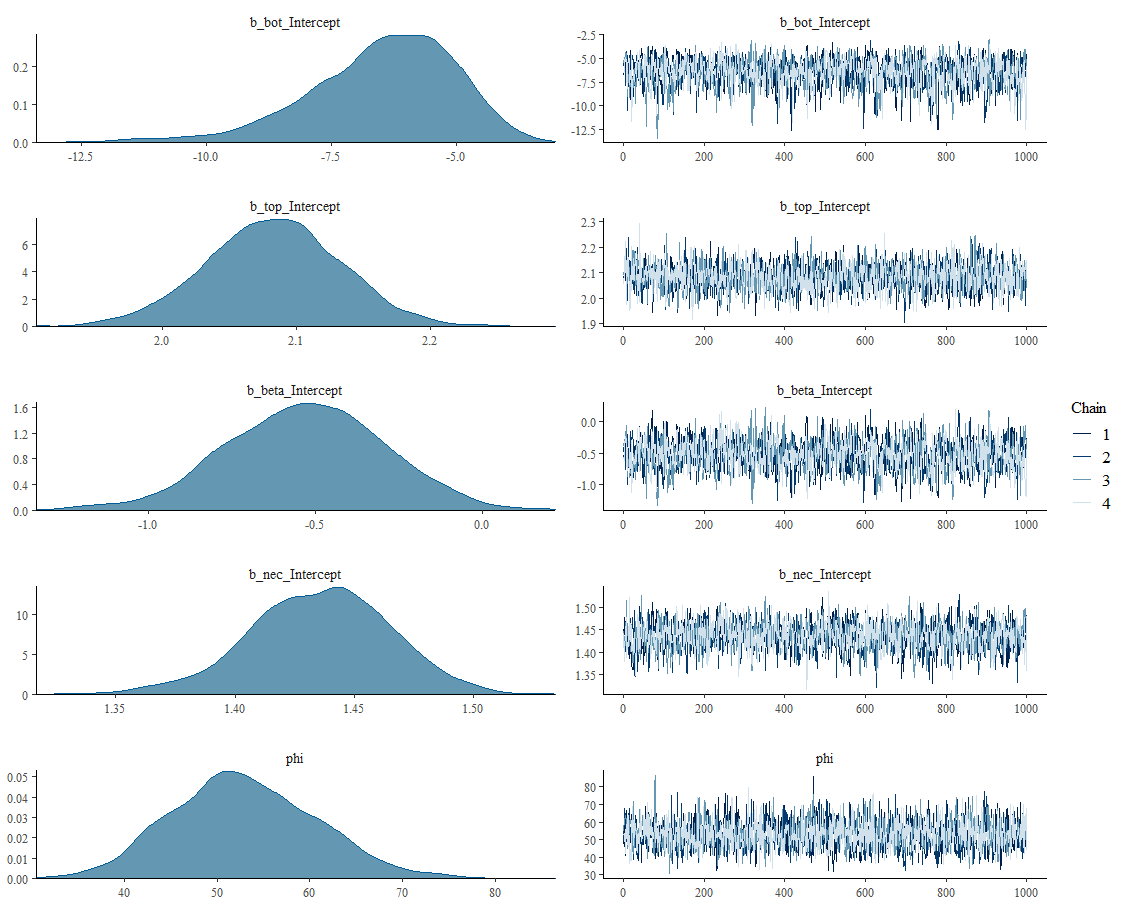
\includegraphics{brms_plot.png}
\caption{Default pkg\{brms\} plot of the \texttt{nec4param} model
showing the posterior probability densities and chain mixing for each of
the included parameters.\label{fig:brmsplot}}
\end{figure}

which yields a plot of the posterior densities and chains plot for each
parameter in the specified model as shown in \autoref{fig:brmsplot}.

The default number of total iterations in pkg\{bayesnec\} is 10,000 per
chain, with 9,000 of these used as warm-up (or burn-in) across 4 chains.
If the \texttt{bnec} call returns pkg\{brms\} warning messages the
number of iterations and warm-up samples can be adjusted through
arguments \texttt{iter} and \texttt{warmup}. A range of other arguments
can be further adjusted to improve convergence, see the rich set of
\href{https://github.com/paul-buerkner/brms}{Resources} available for
the pkg\{brms\} package for further information.

Several helper functions have been included that allow the user to add
or drop models from a \texttt{bayesmanecfit} object, or change the model
weighting method (\texttt{amend}); extract a single or subset of models
from the \texttt{bayesmanecfit} object (\texttt{pull\_out}); and examine
the priors used for model fitting (\texttt{pull\_prior},
\texttt{sample\_priors} and \texttt{check\_priors}).

\hypertarget{model-inference}{%
\subsubsection{Model inference}\label{model-inference}}

pkg\{bayesnec\} includes a summary method for both \texttt{bayesnecfit}
and \texttt{bayesmanecfit} model objects, providing the usual summary of
model parameters and any relevant model fit statistics as returned in
the underlying \texttt{brm} model fits. This includes a list of fitted
models, their respective model weights, and a model-averaged
\emph{NEC}---which is reported with a warning in case it contains NSEC
values. A warning message also indicates that the \textbf{ecxll5} model
may have convergence issues according to the default pkg\{brms\}
\(\widehat{R}\) criteria:

\begin{CodeChunk}
\begin{CodeInput}
R> summary(exmp_fit)
\end{CodeInput}
\begin{CodeOutput}
Object of class bayesmanecfit containing the following non-linear models:
  -  nec4param
  -  nechorme4
  -  neclin
  -  neclinhorme
  -  nechorme4pwr
  -  ecxlin
  -  ecx4param
  -  ecxwb1
  -  ecxwb2
  -  ecxll5
  -  ecxll4
  -  ecxhormebc5

Distribution family: beta
Number of posterior draws per model:  4000

Model weights (Method: pseudobma_bb_weights):
                waic   wi
nec4param    -333.21 0.26
nechorme4    -332.41 0.16
neclin       -332.74 0.27
neclinhorme  -331.05 0.13
nechorme4pwr -331.36 0.09
ecxlin       -187.92 0.00
ecx4param    -302.15 0.00
ecxwb1       -294.71 0.00
ecxwb2       -316.85 0.00
ecxll5       -331.03 0.08
ecxll4       -302.00 0.00
ecxhormebc5  -309.78 0.00


Summary of weighted NEC posterior estimates:
NB: Model set contains the ECX models: ecxlin;ecx4param;ecxwb1;ecxwb2;ecxll5;ecxll4;ecxhormebc5; weighted NEC estimates include NSEC surrogates for NEC
    Estimate Q2.5 Q97.5
NEC     1.40 1.28  1.48
\end{CodeOutput}
\end{CodeChunk}

Base R (\texttt{plot}) and ggplot2 (\texttt{ggbnec}) plotting methods,
as well as predict methods have also been developed for both
\texttt{bayesnecfit} and \texttt{bayesmanecfit} model classes. In
addition, there are method-based functions for extracting \emph{ECx}
(\texttt{ecx}), \emph{NEC} (\texttt{nec}) and \emph{NSEC}
(\texttt{nsec}) threshold values. In all cases the posterior samples
that underpin these functions are achieved through
\texttt{posterior\_epred} from the pkg\{brms\} package. An example base
plot of a \texttt{bayesmanecfit} model fit can be seen in
\autoref{fig:baseplot}.

\begin{CodeChunk}
\begin{CodeInput}
R> plot(exmp_fit)
\end{CodeInput}


\begin{center}\includegraphics{article_files/figure-latex/base-plot-1} \end{center}

\end{CodeChunk}

\begin{figure}
\centering
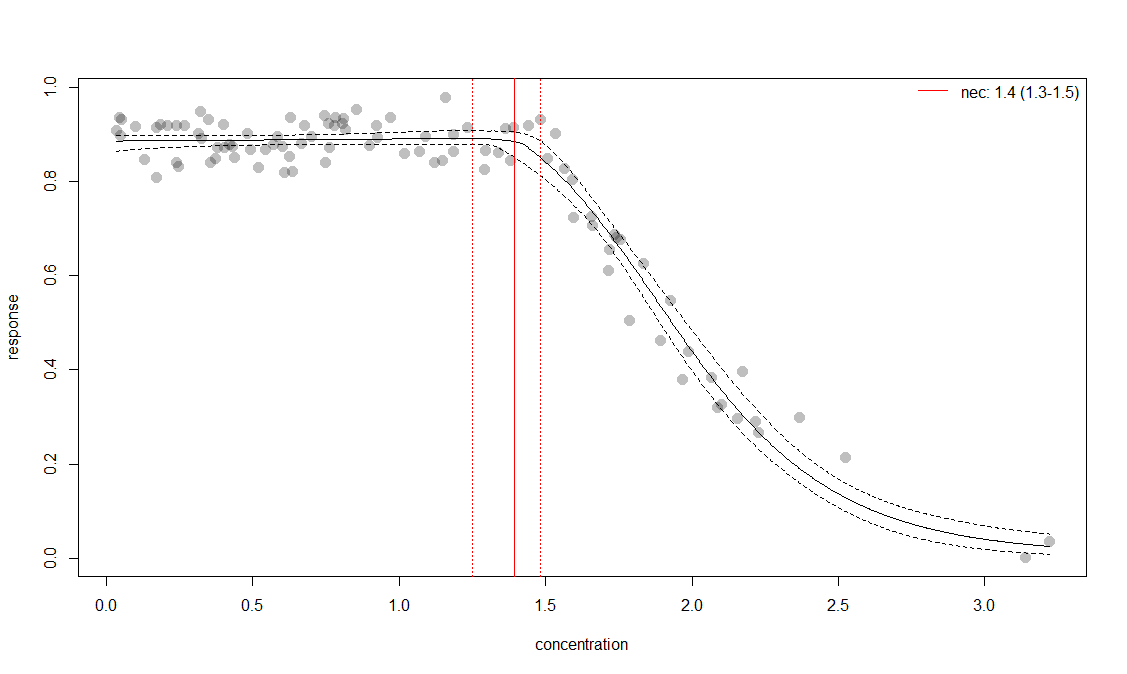
\includegraphics{base_plot.png}
\caption{Base plot of the \texttt{exmp\_fit} model averaged curve,
showing the fitted median of the posterior prediction (solid line), 95\%
credible intervals (dashed lines), and the estimated \emph{NEC} value
(red vertical lines).\label{fig:baseplot}}
\end{figure}

By default the plot shows the fitted posterior curve with 95\% credible
intervals, along with an estimate of the \(\eta = \text{NEC}\) value.
Please see the
\href{https://open-aims.github.io/bayesnec/articles/}{vignettes} for
more examples using pkg\{bayesnec\} models for inference.

\hypertarget{models-in-pkgbayesnec}{%
\subsection{Models in pkg\{bayesnec\}}\label{models-in-pkgbayesnec}}

The argument \texttt{model} in the function \texttt{bnec} is a character
string indicating the name(s) of the desired model. If a recognised
model name is provided, a single model of the specified type is fit, and
\texttt{bnec} returns a model object of class \texttt{bayesnecfit}. If a
vector of two or more of the available models are supplied,
\texttt{bnec} returns a model object of class \texttt{bayesmanecfit}
containing Bayesian model averaged predictions for the supplied models,
providing they were successfully fitted.

The \texttt{model} argument may also be one of ``all'', meaning all of
the available models will be fit; ``ecx'' meaning only models excluding
the \(\eta = \text{NEC}\) step parameter will be fit; or ``nec'' meaning
only models with the \(\eta = \text{NEC}\) step parameter (see below
\textbf{Model parameters}) will be fit. There are a range of other
pre-defined model groups available. The full list of currently
implemented model groups can be seen using the function
\texttt{models()}.

Please see the
\href{https://open-aims.github.io/bayesnec/articles/example2b.html}{Model
details} vignette or \texttt{?model("all")} for more information on all
the models available in pkg\{bayesnec\} and their specific formulation.

\hypertarget{parameter-definitions}{%
\subsubsection{Parameter definitions}\label{parameter-definitions}}

Where possible we have aimed for consistency in the interpretable
meaning of the individual parameters across models. Across the currently
implemented model-set, models contain from two (basic linear or
exponential decay, see \textbf{ecxlin} or \textbf{ecxexp}) to five
possible parameters (e.g.~\textbf{nechorme4}, \textbf{ecxhormebc5}),
including:

\begin{itemize}
\item
  \(\tau = \text{top}\), usually interpretable as either the y-intercept
  or the upper plateau representing the mean concentration of the
  response at zero concentration;
\item
  \(\eta = \text{NEC}\), the no-effect-concentration value (the x
  concentration value where the breakpoint in the regression is
  estimated at, see \textbf{Model types for \emph{NEC} and \emph{ECx}
  estimation} and \citep{Fox2010} for more details on parameter based
  \emph{NEC} estimation);
\item
  \(\beta = \text{beta}\), generally the exponential decay rate of
  response, either from 0 concentration or from the estimated \(\eta\)
  value, with the exception of the \textbf{neclinhorme} model where it
  represents a linear decay from \(\eta\) because slope (\(\alpha\)) is
  required for the linear increase;
\item
  \(\delta = \text{bottom}\), representing the lower plateau for the
  response at infinite concentration;
\item
  \(\alpha = \text{slope}\), the linear decay rate in the models
  \textbf{neclin} and \textbf{ecxlin}, or the linear increase rate prior
  to \(\eta\) for all hormesis models;
\item
  \(\text{ec50}\) notionally the 50\% effect concentration but may be
  influenced by scaling and should therefore not be strictly
  interpreted; and
\item
  \(\epsilon = \text{d}\), the exponent in the \textbf{ecxsigm} and
  \textbf{necisgm} models.
\end{itemize}

In addition to the model parameters, all \texttt{nec...} models have a
step function used to define the breakpoint in the regression, which can
be defined as:

\[
f(x_i, \eta) = \begin{cases} 
      0, & x_i - \eta < 0 \\
      1, & x_i - \eta \geq 0 \\
   \end{cases}
\]

\hypertarget{model-types-for-nec-and-ecx-estimation}{%
\subsubsection{\texorpdfstring{Model types for \emph{NEC} and \emph{ECx}
estimation}{Model types for NEC and ECx estimation}}\label{model-types-for-nec-and-ecx-estimation}}

All models provide an estimate of the no-effect-concentration
(\emph{NEC}). For model types with ``nec'' as a prefix, the \emph{NEC}
is directly estimated as parameter \(\eta = \text{NEC}\) in the model,
as per \citet{Fox2010}. Models with ``ecx'' as a prefix are continuous
curve models, typically used for extracting \emph{ECx} values from C-R
data. In this instance the \emph{NEC} reported is actually the
no-significant-effect-concentration (\emph{NSEC}), defined as the
concentration at which the predicted response is now ``significantly''
lower than the values observed at the lowest treatment concentration
(typically the `control'). The desired level of ``significance'' can be
controlled by the user through the argument \texttt{sig\_val}, which is
passed as a probability to \texttt{quantile} and used to calculate the
lower bound of the posterior predictions at the lowest treatment
concentration. The default value for \texttt{sig\_val} is 0.01, which is
analogous to an alpha value (Type 1 error rate) of 0.01 for a one-sided
test of significance. See \texttt{?nsec} for more details. We currently
recommend only using the ``nec'' model-set for estimation of \emph{NEC}
values, as the \emph{NSEC} concept has yet to be formally peer-reviewed,
and likely suffers from at least some of the same issues as the
No-observed-effect-concentration (\emph{NOEC},
\citep{Warne2008a, Fox2008}).

\emph{ECx} estimates can be equally validly obtained from both ``nec''
and ``ecx'' models. \emph{ECx} estimates will usually be lower (more
conservative) for ``ecx'' models fitted to the same data as ``nec''
models (see the
\href{https://open-aims.github.io/bayesnec/articles/example4.html}{Comparing
posterior predictions} vignette for an example. However, we recommend
using ``all'' models where \emph{ECx} estimation is required because
``nec'' models can fit some datasets better than ``ecx'' models and the
model averaging approach will place the greatest weight for the outcome
that best fits the supplied data. This approach will yield \emph{ECx}
estimates that are the most representative of the underlying
relationship in the dataset.

There is ambiguity in the definition of \emph{ECx} estimates from
hormesis models (these allow an initial increase in the response
\citep[see][]{Mattson2008} and include models with the character string
\texttt{horme} in their name), as well as those that have no natural
lower bound on the scale of the response (models with the string
\texttt{lin} in their name, in the case of Gaussian response data). For
this reason, the \texttt{ecx} function has arguments
\texttt{hormesis\_def} and \texttt{type}, both character vectors
indicating the desired behaviour. For \texttt{hormesis\_def\ =\ "max"}
\emph{ECx} values are calculated as a decline from the maximum estimates
(i.e.~the peak at \(\eta = \text{NEC}\)); and
\texttt{hormesis\_def\ =\ "control"} (the default) indicates \emph{ECx}
values should be calculated relative to the control, which is assumed to
be the lowest observed concentration. For \texttt{type\ =\ "relative"}
\emph{ECx} is calculated as the percentage decrease from the maximum
predicted value of the response (\(\tau = \text{top}\)) to the minimum
predicted value of the response (ie, `relative' to the observed data).
For \texttt{type\ =\ "absolute"} (the default) \emph{ECx} is calculated
as the percentage decrease from the maximum value of the response
(\(\tau = \text{top}\)) to 0 (or \(\delta = \text{bottom}\) for models
with that parameter). For \texttt{type\ =\ "direct"}, a direct
interpolation of y on x is obtained.

\hypertarget{model-suitability-for-response-types}{%
\subsubsection{Model suitability for response
types}\label{model-suitability-for-response-types}}

Models that have an exponential decay (most models with parameter
\(\beta = \text{beta}\)) with no \(\delta = \text{bottom}\) parameter
are 0 bounded and are not suitable for the Gaussian family, or any
family modelled using a logit or log link because they cannot generate
predictions of negative y (response). Conversely models with a linear
decay (containing the string \texttt{lin} in their name) are not
suitable for modelling families that are 0 bounded (Gamma, Poisson,
Negative-binomial, Beta, Binomial, Beta-binomial) using an identity
link. These restrictions do not need to be controlled by the user as a
call to \texttt{bnec} with \texttt{models\ =\ "all"} will simply exclude
inappropriate models, albeit with a message.

Strictly speaking, models with a linear hormesis increase are not
suitable for modelling data from the Binomial, Beta and Beta-binomial
families, however they are currently allowed in pkg\{bayesnec\}, with a
reasonable fit achieved through a combination of the appropriate family
being applied to the response, and the pkg\{bayesnec\}
\texttt{make\_inits} function that ensures initial values passed to
pkg\{brms\} yield response values within the range of the observed
\texttt{y\_var} data.

\hypertarget{priors-on-model-parameters}{%
\subsection{Priors on model
parameters}\label{priors-on-model-parameters}}

In Bayesian inference, model parameters and their inherent uncertainty
are estimated as statistical probability distributions. This is achieved
by combining an a-prior understanding of each parameter's probability
density function (the `priors') with the likelihood of the observed
information (data) given the model parameters, to yield a so-called
posterior probability distribution. Regardless of whether this is done
mathematically via Bayes' theorem or through Monte Carlo simulation, to
carry out a Bayesian analysis the prior probability densities must be
defined. Sometimes there may be substantial prior knowledge, for example
when pilot data or data from a previous experiment exist for a given
response curve. In this case the prior probability distribution may be
quite narrow (highly ``informative'') and can have a strong influence on
the posterior, especially when subsequent data are scarce or highly
variable. In our experience however, such prior knowledge is generally
the exception. Where no quantitative prior information exists, it is
common in Bayesian statistics to use ``vague'' or ``weakly'' informative
priors. The use of ``vague'', ``diffuse'', ``flat'' or otherwise
so-called ``uninformative'' priors is no longer recommended
\citep{Banner2020}. Such priors generally form the default for many
Bayesian packages, and are often used in practice without critical
thought or evaluation, possibly as a result of fear of being too
`subjective' \citep{Banner2020}.

Considerable thought has gone into development of an algorithm
(\texttt{define\_prior}) to build ``weakly'' informative priors for
fitting models in pkg\{bayesnec\}. The priors are ``weakly'' informative
in that in addition to specifying the relevant statistical family that
appropriately captures the parameters likely theoretical statistical
distribution, we also use information contained within the observed data
to centre the probability density near the most likely parameter space
and/or constrain priors to sensible bounds. These weakly informative
priors are used to help constrain the underlying routines so that they
are less likely to consider what the researcher would deem highly
improbable estimates, that also cause the routines to become unstable.
Weakly informative priors can be particularly helpful in complex
non-linear modelling to ensure reliable convergence. These types of
priors specify the general shape and bounds of the expected probability
distribution for a given parameter, whilst remaining sufficiently broad
so as not to influence the parameter's estimated posterior distribution
(given a reasonable amount of observed data). In this sense
appropriately weak priors should yield analytical outcomes that share
the same level of \emph{objectivity} as equivalent frequentist
approaches, whilst yielding robust parameter estimates with
probabilistically interpretable uncertainty bounds. To ensure a
pkg\{bayesnec\} analysis retains the same level of objectivity as an
equivalent frequentist approach we recommend using the function
\texttt{check\_priors} to compare the prior and posterior probability
densities and check that the priors used by pkg\{bayesnec\} are sensible
and are not exerting an undesirable influence over the analysis.

\hypertarget{pkgbayesnecs-define_prior-algorithm}{%
\subsubsection{\texorpdfstring{pkg\{bayesnec\}'s \texttt{define\_prior}
algorithm}{pkg\{bayesnec\}'s define\_prior algorithm}}\label{pkgbayesnecs-define_prior-algorithm}}

Priors are constructed in pkg\{bayesnec\} for each parameter of each
model being fitted based on the characteristics of either the input
\texttt{x\_var} or \texttt{y\_var} data, depending on which is relevant
to the specific parameter scaling. In the case of parameters that scale
with \texttt{y\_var} (the response), priors are constructed based on the
relevant link scaling, whether that be identity, the default (for that
family), or user specified link function for a specific family. The
priors are constructed by \texttt{bnec} internally calling the function
\texttt{define\_prior}, which takes the arguments \texttt{model},
\texttt{family} (including the relevant link function),
\texttt{predictor} (\texttt{x\_var} data), and \texttt{response}
(\texttt{y\_var} data).

\hypertarget{priors-for-response-y_var-scaled-parameters}{%
\paragraph{\texorpdfstring{Priors for response (\texttt{y\_var}) scaled
parameters}{Priors for response (y\_var) scaled parameters}}\label{priors-for-response-y_var-scaled-parameters}}

Only the parameters \(\tau = \text{top}\) and \(\delta = \text{bottom}\)
scale specifically with the response (\texttt{y\_var} data) family. For
Gaussian \texttt{y\_var} data (or any \texttt{y\_var} data for which the
link ensures valid values of the response can take from -\(\infty\) to
\(\infty\), including \texttt{log} and \texttt{logit}) priors are
Gaussian with a standard deviation of 2.5 and a mean set at the
90\textsuperscript{th} and 10\textsuperscript{th} quantiles for
\(\tau = \text{top}\) and \(\delta = \text{bottom}\) respectively. In
this way pkg\{bayesnec\} attempts to construct a prior that scales
appropriately with the observed data, with greatest density near the
most likely region of the response for the \(\tau = \text{top}\) and
\(\delta = \text{bottom}\) parameters, whilst remaining broad enough to
have little influence on each parameter's posterior density.

For Poisson-, Negative-binomial- and Gamma-distributed \texttt{y\_var}
data, the response is bounded by 0 and therefore Gaussian priors are
unsuitable. Instead we use Gamma priors, with a mean scaled to
correspond to the 75\textsuperscript{th} and 25\textsuperscript{th}
quantiles for \(\tau = \text{top}\) and \(\delta = \text{bottom}\)
respectively. The mean (\(\mu\)) is linked mathematically to the shape
(s) and rate parameters (r) by the equation \[ \mu = s * (1/r) \] with
the shape parameter being set to 2 by default.

For the Binomial, Beta, and Beta-binomial families, estimates for
\(\tau = \text{top}\) and \(\delta = \text{bottom}\) must necessarily be
constrained between 0 and 1 when modelled on the identity link. Because
of this constraint there is no need to adjust scaling based on the
response. In this case pkg\{bayesnec\} uses \texttt{beta(5,\ 1)} and
\texttt{beta(1,\ 5)} priors to provide a broad density centred across
the upper and lower 0 to 1 range for the \(\tau = \text{top}\) and
\(\delta = \text{bottom}\) parameters respectively.

\hypertarget{priors-for-predictor-x_var-scaled-parameters}{%
\paragraph{\texorpdfstring{Priors for predictor (\texttt{x\_var}) scaled
parameters}{Priors for predictor (x\_var) scaled parameters}}\label{priors-for-predictor-x_var-scaled-parameters}}

The parameters \(\eta = \text{NEC}\) and \(\eta = \text{ec50}\) scale
with respect to the predictor (\texttt{x\_var} data), because both of
these are estimated in units of the predictor (\texttt{x\_var}, usually
concentration). To stabilise model fitting, the \(\eta = \text{NEC}\)
and \(\eta = \text{ec50}\) parameters are bounded to the upper and lower
observed range in the predictor, under the assumption that the range of
concentrations in the experiment were sufficient to cover the full range
of the response outcomes. The priors used reflect the characteristics of
the observed data that are used to predict the appropriate family. If
the \texttt{x\_var} data are bounded to 0 and \textgreater1 a Gamma
prior is used, with maximum density (\(\mu\), see above) at the median
value of the predictor, and a shape parameter of 5. If the
\texttt{x\_var} data are bounded to 0 and 1 a \texttt{beta(2,\ 2)} prior
is used. For \texttt{x\_var} data ranging from -\(\infty\) to
\(\infty\), a Gaussian prior is used, with a mean set at the median of
the \texttt{x\_var} values and a standard deviation of 2.5.

\hypertarget{priors-for-other-parameters}{%
\paragraph{Priors for other
parameters}\label{priors-for-other-parameters}}

For the parameters \(\beta = \text{beta}\), \(\alpha = \text{slope}\)
and \(\epsilon = \text{d}\) we first ensured any relevant
transformations in the model formula such that theoretical values with
the range -\(\infty\) to \(\infty\) are allowable, and a
\texttt{normal(0,\ 2)} prior is used. For example in the
\texttt{nec3param} model \(\beta = \text{beta}\) is an exponential decay
parameter, which must by definition be bounded to 0 and \(\infty\).
Calling \texttt{exp(beta)} in the model formula ensures the exponent
meets these requirements. Note also that a mean of 0 and standard
deviation of 2 represents a relatively broad prior on this exponential
scaling, so this is still generally a weakly informative prior in
practice.

\hypertarget{user-specified-priors}{%
\subsubsection{User specified priors}\label{user-specified-priors}}

There may be situations where the default pkg\{bayesnec\} priors do not
behave as desired, or the user wants to provide informative priors. For
example, the default priors may be too informative, yielding
unreasonably tight confidence bands (although this is only likely where
there are few data or unique values of the \texttt{x\_var} data).
Conversely, priors may be too vague, leading to poor model convergence.
Alternatively, the default priors may be of the wrong statistical family
if there was insufficient information in the provided data for
pkg\{bayesnec\} to correctly predict the appropriate ones to use. The
priors used in the default model fit can be extracted using
\texttt{pull\_prior}, and a sample or plot of prior values can be
obtained from the individual pkg\{brms\} model fits through the function
\texttt{sample\_priors} which samples directly from the \texttt{prior}
element in the \texttt{brm} model fit (see \autoref{fig:priorsplot}).

\begin{CodeChunk}
\begin{CodeInput}
R> sample_priors(exmp_fit$mod_fits$nec4param$fit$prior)
\end{CodeInput}


\begin{center}\includegraphics{article_files/figure-latex/sample-prior-1} \end{center}

\end{CodeChunk}

\begin{figure}
\centering
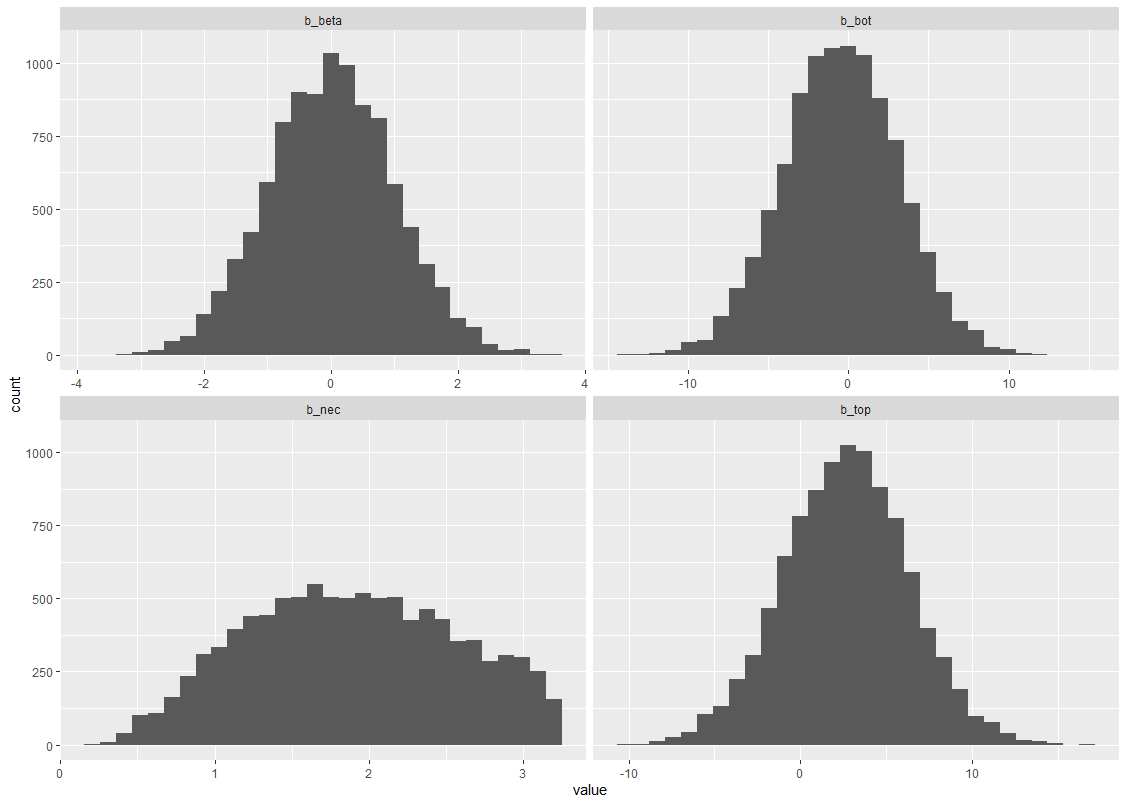
\includegraphics{sample_prior.png}
\caption{Frequency histograms of samples of the default priors used by
\texttt{bnec} for fitting the \texttt{nec4param} model to the example
\texttt{nec\_data}.\label{fig:priorsplot}}
\end{figure}

We can also use the function \texttt{check\_priors} (based on the
\texttt{hypothesis} function of pkg\{brms\}) to assess how the posterior
probability density for each parameter differs from that of the prior.
Here we show the prior and posterior probability densities for the
parameters in the \textbf{nec4param} model, extracted from our example
fit (see \autoref{fig:checkpriorsplot}). There is also a class
\texttt{bayesmanecfit} method that can be used to sequentially view all
plots in a \texttt{bnec} call with multiple models, or write to a pdf as
in \texttt{check\_chains}.

This can be done for a single model using:

\begin{CodeChunk}
\begin{CodeInput}
R> exmp_fit_nec4param <- pull_out(exmp_fit, model = "nec4param")
R> check_priors(exmp_fit_nec4param)
\end{CodeInput}


\begin{center}\includegraphics{article_files/figure-latex/check-priorsingle-1} \end{center}

\end{CodeChunk}

or for all models, writing to a pdf file named Check\_priors\_plots.pdf:

\begin{CodeChunk}
\begin{CodeInput}
R> check_priors(exmp_fit, filename = "Check_priors_plots")
\end{CodeInput}
\end{CodeChunk}

\begin{figure}
\centering
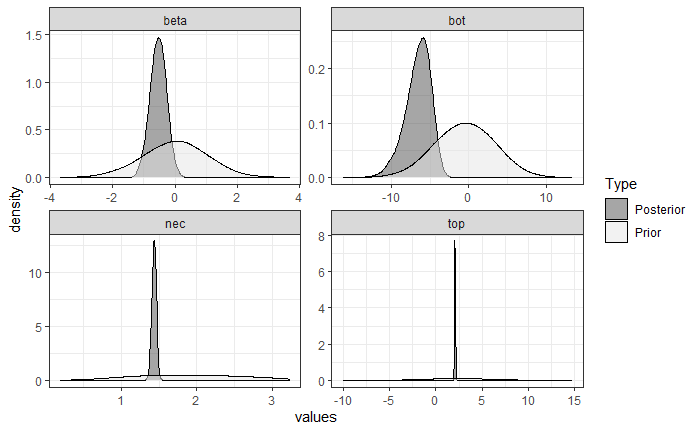
\includegraphics{check_prior.png}
\caption{A comparison of the prior and posterior parameter probability
densities for the \texttt{nec4param} model fit to the example
\texttt{nec\_data}.\label{fig:checkpriorsplot}}
\end{figure}

\hypertarget{model-comparison}{%
\subsection{Model comparison}\label{model-comparison}}

With pkg\{bayesnec\} we have included a function
(\texttt{compare\_posterior}) that allows bootstrapped comparisons of
posterior predictions. This function allows the user to fit several
different \texttt{bnec} model fits and compare differences in the
posterior predictions. Comparisons can be made across the model fits for
individual endpoint estimates (e.g.~\emph{NEC}, \emph{NSEC} or
\emph{ECx}) or across a range of predictor (x) values. Usage is
demonstrated in the relevant
\href{https://open-aims.github.io/bayesnec/articles/example4.html}{vignette}
by comparing different types of models and model-sets using a single
dataset. However, the intent of this function is to allow comparison
across different datasets that might represent, for example, different
levels of a fixed factor covariate. For example, this function has been
used to compare toxicity of herbicides across three different climate
scenarios, to examine the cumulative impacts of pesticides and global
warming on corals \citep{flores2021}.

At this time \texttt{bnec} does not allow for an inclusion of an
interaction with a fixed factor. Including an interaction term within
each of the non-linear models implemented in pkg\{bayesnec\} is
relatively straightforward, and may be introduced in future releases.
However, in many cases the functional form of the response may change
with different levels of a given factor. The substantial complexity of
defining all possible non-linear model combinations at each factor level
means it unlikely this could be feasibly implemented in pkg\{bayesnec\}
in the short term. In the meantime the greatest flexibility in the
functional form of individual model fits can be readily obtained using
models fitted independently to data within each factor level.

\hypertarget{random-effects}{%
\subsection{Random effects}\label{random-effects}}

Most eco-toxicological and toxicology experiments include a range of
grouping elements, such as tanks, vials or batches of samples that
contain multiple measurements that cannot be considered strictly
independent (aka they are pseudo-replicates). To avoid criticism around
potential issues with pseudo-replication, it is often the practice for
ecotoxicologists to pool such observations and carry out modelling
using, for example, the group mean. Where the number of within group
observations varies substantially across groups, this will have the
undesirable effect of equally weighting the group means even though some
may be based on far fewer observations than others. In addition there
are often instances of ecotoxicology data from multiple experiments or
other grouping factors within an experiment (such as genotype) that
cover the full range of x concentrations that cannot be averaged prior
to modelling, resulting in the ecotoxicologist either ignoring the
potential non-independence, or fitting many independent datasets and
subsequently needing to aggregate the endpoint estimates. Carrying out
multiple fits on separate datasets is undesirable because each fit is
based on fewer data and will have greater uncertainty.

The current version of pkg\{bayesnec\} allows a list of random terms to
be passed through the argument \emph{random} to pkg\{brms\} for
accommodating hierarchical designs and other forms of non-independence.
Random effects can be in the form of a random offset, which effectively
allows different mean response levels across groups, and is achieved
through specifying the random term ``ost'' in the named list. Random
effects can also be added to any or all of the non-linear parameters in
the model. Note that implementing random effects in a non-linear
modelling setting is non-trivial and considerable thought and testing
should go into selecting an appropriate random structure.

\hypertarget{discussion-and-caveats}{%
\section{Discussion and caveats}\label{discussion-and-caveats}}

In order to be accessible to a broad community of varying statistical
capabilities, we have simplified fitting a pkg\{bayesnec\} model as much
as possible, whilst retaining the ability to modify a wide range of
arguments as necessary. Where possible we have tried to set default
values to align with those in pkg\{brms\}. Wherever we deviate, this is
generally towards being more conservative and/or we have clearly
explained our reasoning. Specific examples include: 1) \texttt{iter},
which we increased from the pkg\{brms\} default of 2,000 to 10,000 as we
found that a higher number of MCMC iterations are generally required for
these sometimes complex non-linear models; 2) the use of pseudo-BMA
rather than stacking weights to better reflect pkg\{bayesnec\}'s goals
with respect to model averaging (discussed in more detail above); and 3)
the use of \texttt{pointwise\ =\ TRUE} (where possible) and
\texttt{sample\_prior\ =\ "yes"} to avoid excessive R crashes when used
in the Windows operating system and allow the use of the
\texttt{hypothesis} function respectively. We welcome constructive
criticism of our selections and users must expect that default settings
may change accordingly in later releases.

We have made considerable effort to ensure that pkg\{bayesnec\} makes a
sensible prediction for the appropriate family, constructs appropriate
weakly informative priors, and generates sensible initial values.
However, this is a difficult task across such a broad range of
non-linear models, and across the potential range of ecotoxicological
data that may be used. The user must interrogate their model fits using
the wide array of helper functions, and use their own judgement
regarding the appropriateness of model inferences for their own
application. Of particular importance are examination of model fit
statistics through the \texttt{summary} and \texttt{rhat} methods,
visual inspection of all model fits in \texttt{bayesmanecfit} objects
(via \texttt{plot(...,\ all\_models\ =\ TRUE)} and
\texttt{check\_chains(...,\ all\_models\ =\ TRUE)}) and an assessment of
the posterior versus prior probability densities to ensure default
priors are appropriate.

The model averaging approach implemented in pkg\{bayesnec\} is widely
used in a range of settings \citep[in ecology for example, see][ for a
thorough review]{Dormann2018}. However, model averaging is relatively
new to ecotoxicology \citep[but see, for
example,][]{Shao2014, Thorley2018, fox2020, Wheeler2009}. In
pkg\{bayesnec\} we have implemented a broad range of potential models,
and the default behaviour is to fit them all, although we discuss above
situations where this is clearly not recommended (for example, in the
estimation of \textbf{NEC}). More research is required to understand how
model-set selection influences model inference. While some studies
suggest using a broad range of models may be optimal
\citep{Wheeler2009}, others indicate that including multiple models of
similar shape may overweight the representation of that shape in model
averaged predictions \citep{fox2020}. In addition, it is important to
understand that when models are added or removed from the model-set,
this can sometimes have a substantial influence on model predictions
(potentially changing estimated \textbf{ECx} values, for example). As
the model-set in pkg\{bayesnec\} may change through time it is important
to keep a record of the models that were actually fitted in a given
analysis, in the event it is necessary to reproduce a set of results. A
potentially better strategy is to build a
\href{https://docs.docker.com/get-docker/}{Docker} container, an
emerging approach representing one strategy towards overcoming the
reproducibility crisis \citep{Baker2016}. Considerations of analytical
reproducibility are particularly relevant to C-R modelling, where the
model outcomes can often have far reaching management implications.

Like R itself, pkg\{bayesnec\} is free software and comes with
ABSOLUTELY NO WARRANTY, or even IMPLIED WARRANTY.

\hypertarget{future-directions}{%
\section{Future directions}\label{future-directions}}

The pkg\{bayesnec\} package is a work in progress, and we welcome
suggestions and feedback that will improve the package performance and
function. Our goal is to make pkg\{bayesnec\} as user friendly as
possible, and capable of dealing with most real world C-R modelling
applications in the hope that Bayesian statistics will become more
widely used in applied risk assessment. Please submit requests through
the package \href{https://github.com/open-AIMS/bayesnec/issues}{Issues}
on github. Some suggested future enhancements include:

\begin{itemize}
\item
  The addition of other custom families, such as the tweedie
  distribution. Currently pkg\{bayesnec\} implements adjustments away
  from 0 (Gamma, Beta) or 1 (Beta) as a strategy for allowing modelling
  with these types of data using the closest most convenient statistical
  distribution. To our knowledge there are no readily available
  distributions able to model data that includes 0 and 1 on the
  continuous scale, and 0 and 1 adjustments followed by modelling using
  a Beta distribution remains the most appropriate option. For data that
  are 0 to \(\infty\) on the continuous scale the Tweedie distribution
  may prove a much better option than the current zero bounded Gamma,
  and has been used extensively in fisheries research for biomass data
  \citep{Shono2008}. As this family is not currently available in
  pkg\{brms\} this would need to be implemented as a custom family,
  which for the Tweedie is not trivial.
\item
  A hypothesis method for testing against toxicity thresholds. The
  pkg\{brms\} package includes a \texttt{hypothesis} function that
  allows for testing parameter estimates against specified criteria.
  This is used in pkg\{bayesnec\} in the \texttt{check\_prior} function,
  which is a wrapper that examines the deviation of each parameter in
  the given model relative to 0 as a means of generating posterior and
  prior probability density plots for comparison. However, an additional
  wrapper function could be developed that allows toxicity to be
  assessed, as measured through \emph{NEC}, or \emph{ECx} for example,
  against a required pre-defined threshold. Such a feature may be useful
  where toxicity testing is used as a trigger in risk management.
\end{itemize}

\hypertarget{acknowledgements}{%
\section{Acknowledgements}\label{acknowledgements}}

The development of pkg\{bayesnec\} was supported by an AIMS internal
grant. David Fox and Gerard Ricardo developed some of the initial code
on which the pkg\{bayesnec\} predecessor pkg\{jagsNEC\} was based.
Usage, testing and functionality of both the pkg\{jagsNEC\} and
pkg\{bayesnec\} packages were substantially aided through input from
Joost van Dam, Andrew Negri, Florita Flores, Heidi Luter, Marie Thomas
and Mikaela Nordborg. Florita Flores and Murray Logan provided valuable
comments on the manuscript text. Ron Jones resolved issues with the
paper.bib file that was causing compilation to fail.

\renewcommand\refname{References}
\bibliography{refs.bib}


\end{document}
